% ថ្នាក់ទី ១១ (វិទ្យាសាស្ត្រសង្គម) · ជំពូកទី ៦ · មេរៀនទី ៣ · សៀវភៅ ទំព័រ ២៣៨–២៦៦
\chapter{ប្រូបាប}

\begin{objBox}[វត្ថុបំណង]
\begin{enumerate}[1]
  \item កំណត់ន័យរបស់ពាក្យ ពិសោធន៍ចៃដន្យ វិញ្ញាសា លំហសំណាក និងព្រឹត្តិការណ៍
  \item បង្ហាញប្រភេទនៃព្រឹត្តិការណ៍ឯកធាតុ ព្រឹត្តិការណ៍សមាស ព្រឹត្តិការណ៍ប្រាកដ ព្រឹត្តិការណ៍មិនអាចមាន ព្រឹត្តិការណ៍ផលបូក ផលគុណ ព្រឹត្តិការណ៍មិនចុះសម្រុងនិងផ្ទុយ
  \item កំណត់និយមន័យប្រូបាប រូបមន្ត និងលក្ខណៈនៃប្រូបាប
  \item ប្រើរូបមន្តចម្លាស់និងបន្សំ ដើម្បីគណនាប្រូបាបនៃព្រឹត្តិការណ៍មួយ ។
\end{enumerate}
\end{objBox}

\section{លំហសំណាកនិងព្រឹត្តិការណ៍}
\subsection{ពិសោធន៍ចៃដន្យ-វិញ្ញាសា}

\begin{example}[ឧទាហរណ៍ ១]
នៅពេលដែលគេបោះកាក់មួយ គេមិនអាចដឹងច្បាស់ជាមុនថាកាក់នោះផ្ងារឡើងខាងរូប $(H)$ ឬមួយក៏ខាងលេខ $(T)$ នោះទេ ។ នៅពេលដែលគេបោះគ្រាប់ឡុកឡាក់មួយគ្រាប់ គេក៏មិនអាចដឹងជាមុនថាមុខលើនៃគ្រាប់ឡុកឡាក់ តាងឱ្យលេខណាមួយក្នុងចំណោមលេខពី $1$ ដល់ $6$ ដែរ ។
\end{example}
ពិសោធន៍មួយដែលគេធ្វើដោយមិនបានដឹងជាមុនថា មានលទ្ធផលអ្វីមួយប្រាកដកើតឡើង នោះហៅថា \textbf{ពិសោធន៍ចៃដន្យ} ។

\begin{example}[ឧទាហរណ៍ ២]
បើគេយកកាក់មួយគ្រាប់មកពិសោធន៍ដោយកំណត់ជាក់លាក់ថា គេបោះកាក់ $1$ ដង ឬ $2$ ដង ឬ $3$ ដង $\dots$ នោះគេថា គេធ្វើវិញ្ញាសាបោះកាក់មួយគ្រាប់ចំនួន $1$ ដង ឬ $2$ ដង ឬ $3$ ដង $\dots$ ។
\end{example}

\begin{example}[ឧទាហរណ៍ ៣]
បើគេដាក់សន្លឹកប័ណ្ណ $4$ សន្លឹកចុះលេខ $1, 2, 3$ និង $4$ ក្នុងថង់មួយ រួចគេធ្វើពិសោធន៍ដោយកំណត់សកម្មភាពជាក់លាក់ថា គេចាប់យកប័ណ្ណម្ដងមួយៗចំនួន $2$ លើកចេញពីថង់ដោយចៃដន្យ ហើយមិនដាក់ប័ណ្ណចូលថង់វិញ ។ គេថាគេធ្វើវិញ្ញាសាមួយ គឺវិញ្ញាសាចាប់យកប័ណ្ណចេញពីថង់ម្ដងមួយចំនួន $2$ លើក ដោយមិនដាក់វិញ ។
\end{example}
ពិសោធន៍មួយដែលគេកំណត់ធ្វើដោយជាក់លាក់ក្នុងពិសោធន៍ចៃដន្យមួយហៅថា \textbf{វិញ្ញាសា} ។

\subsection{លំហសំណាក}

\begin{example}[ឧទាហរណ៍]
ក្នុងវិញ្ញាសាបោះកាក់មួយចំនួន $2$ ដង បើលើកទី $1$ គេបោះបានខាងរូបតាងដោយ $H$ និងលើកទី $2$ បានខាងលេខតាងដោយ $T$ នោះគេថាគេបានលទ្ធផល $(HT)$ ។ បើលើកទី $1$ បោះបានខាង $T$ និងលើកទី $2$ បានខាង $T$ នោះគេបានលទ្ធផល $(TT)$ ជាលទ្ធផលដែលបោះបានខាង $T$ ទាំង $2$ លើក ។ តើក្នុងវិញ្ញាសាបោះកាក់មួយ $2$ ដងនេះ គេអាចបានលទ្ធផលទាំងអស់ប៉ុន្មានរបៀប?
\end{example}
លទ្ធផលដែលអាចកើតឡើងទាំងអស់មាន $4$ របៀបគឺ $(HH)$, $(HT)$, $(TH)$ និង $(TT)$ ។
\begin{itemize}
  \item លទ្ធផលទាំងអស់ដែលអាចកើតឡើងក្នុងវិញ្ញាសានេះ បង្កើតបានជាសំណុំមួយហៅថា \textbf{លំហសំណាក} ។ គេកំណត់សរសេរ $S = \{(HH), (HT), (TH), (TT)\}$ ។ ចំនួនលទ្ធផលទាំងអស់តាងដោយ $n(S) = 4$ ។
  \item ក្នុងវិញ្ញាសាបោះកាក់មួយគ្រាប់ចំនួន $1$ ដង គេបានលំហសំណាក $S = \{H, T\}$ ។ ចំនួនលទ្ធផលទាំងអស់តាងដោយ $n(S) = 2$ ។
\end{itemize}

\begin{definition}[និយមន័យ]
\textbf{លំហសំណាក} គឺជាសំណុំលទ្ធផលទាំងអស់ដែលអាចកើតឡើងក្នុងវិញ្ញាសាមួយនៃពិសោធន៍ចៃដន្យ ។ ចំនួនលទ្ធផលក្នុងលំហសំណាកតាងដោយ $n(S)$ ។
\end{definition}

\begin{example}[លំហាត់គំរូ]
គេបោះគ្រាប់ឡុកឡាក់មួយគ្រាប់ចំនួន $2$ ដង ។
\begin{enumerate}[a]
  \item តើសកម្មភាពណាជាពិសោធន៍ចៃដន្យ? ជាវិញ្ញាសា?
  \item សរសេរលំហសំណាក ។
\end{enumerate}
\ans
\begin{enumerate}[a]
  \item ពិសោធន៍ចៃដន្យគឺ សកម្មភាពបោះគ្រាប់ឡុកឡាក់ ។ វិញ្ញាសាគឺ សកម្មភាពបោះគ្រាប់ឡុកឡាក់មួយចំនួន $2$ ដង ។
  \item គេបោះគ្រាប់ឡុកឡាក់មួយចំនួន $2$ ដង លទ្ធផលនីមួយៗដែលអាចកើតឡើងជាគូមានលំដាប់ អាចមានលេខច្រំដែល ដែលជាធាតុរបស់ $E = \{1, 2, 3, 4, 5, 6\}$ ។ គេបានលំហសំណាក ៖ $S = \{(a, b)$ ដែល $a \in E, b \in E\}$
  \[
\begin{aligned}
S &\\
&= \{(1, 1), (1, 2), \dots, (2, 3), (2, 4), \dots, (6, 4), (6, 5), (6, 6)\}
\end{aligned}
\]
  ចំនួនលទ្ធផលដែលអាចកើតឡើងកំណត់ដោយ $n(S) = 6\times 6 = 36$ ករណី ។
\end{enumerate}
\end{example}

\begin{pro}
គេចាប់យកឃ្លីម្ដង $2$ គ្រាប់ចេញពីថង់មួយដោយចៃដន្យ ដែលក្នុងនោះមានឃ្លីក្រហម $2$ ឃ្លីលឿង $2$ និងឃ្លីខៀវ $1$ ។
\begin{enumerate}[a]
  \item តើសកម្មភាពណាជាពិសោធន៍ចៃដន្យ? ជាវិញ្ញាសា?
  \item សរសេរលំហសំណាក ។
\end{enumerate}
\ans
ក. ពិសោធន៍ចៃដន្យ ៖ ការចាប់យកឃ្លីចេញពីថង់ ។ វិញ្ញាសា ៖ ការចាប់យកឃ្លីម្ដង $2$ គ្រាប់ ។ \quad ខ. តាងឃ្លីក្រហម $R_1, R_2$ ឃ្លីលឿង $Y_1, Y_2$ និងឃ្លីខៀវ $B$ ។ លំហសំណាកជាសំណុំនៃគូឃ្លីទាំងអស់ (មិនគិតលំដាប់) ៖ $S = \{R_1R_2, R_1Y_1, R_1Y_2, R_1B, R_2Y_1, R_2Y_2, R_2B, Y_1Y_2, Y_1B, Y_2B\}$, $n(S) = {}_5C_2 = 10$ ។
\end{pro}

\subsection{ព្រឹត្តិការណ៍}
\subsubsection{ព្រឹត្តិការណ៍}

\begin{example}[ឧទាហរណ៍ ១]
ក្នុងវិញ្ញាសាបោះកាក់មួយចំនួន $2$ ដង បើគេកំណត់ថាគេចង់បានខាងរូប $H$ កើតឡើងតែ $1$ ដងគត់ នោះលទ្ធផលដែលស្របនឹងការចង់បាននេះគឺ $(HT)$ និង $(TH)$ ។ បើគេចង់បានខាងរូប $H$ កើតឡើងទាំង $2$ ដង នោះគេបានលទ្ធផល $(HH)$ ។
\end{example}
សំណុំលទ្ធផលដែលកើតឡើងស្របតាមការប្រាថ្នាចង់បានហៅថា \textbf{ព្រឹត្តិការណ៍} ។
\begin{itemize}
  \item បើគេតាង $A$ ជាព្រឹត្តិការណ៍ “បោះកាក់មួយចំនួន $2$ ដង បានខាងរូបម្ដងគត់” នោះគេសរសេរ ៖ $A = \{(HT), (TH)\} \Rightarrow n(A) = 2$ ។
  \item បើគេតាង $B$ ជាព្រឹត្តិការណ៍ “បោះបានខាងលេខ $2$ ដង” ៖ $B = \{(TT)\} \Rightarrow n(B) = 1$ ។
\end{itemize}
ក្នុងវិញ្ញាសានេះ គេឃើញថាលំហសំណាក $S = \{(HH), (HT), (TH), (TT)\} \Rightarrow n(S) = 4$ ។ ដូច្នេះ $A$ និង $B$ ជាសំណុំរងនៃលំហសំណាក ។

\begin{note}[សម្គាល់]
ព្រឹត្តិការណ៍ ជាសំណុំរងនៃលំហសំណាក ។
\end{note}

\begin{example}[ឧទាហរណ៍ ២]
ក្នុងថង់មួយមានឃ្លីក្រហម $1$ ខៀវ $1$ និងលឿង $1$ ។ គេចាប់យកឃ្លីម្ដងមួយៗដោយចៃដន្យចេញពីថង់ រួចដាក់ចូលថង់វិញចំនួន $2$ លើក ។
\end{example}
គេតាង ក ជាឃ្លីពណ៌ក្រហម ខ ជាឃ្លីពណ៌ខៀវ និង ល ជាឃ្លីពណ៌លឿង ។ ក្នុងវិញ្ញាសានេះគេបានលំហសំណាក ៖ $S = \{(a, b)$ ដែល $a, b \in E\}$ ដែល $E = \{\text{ក}, \text{ខ}, \text{ល}\}$
\[
\begin{aligned}
S = \{&(\text{កក}), (\text{ខខ}), (\text{លល}), (\text{កខ}), (\text{ខក}),\\
&(\text{ខល}), (\text{លខ}), (\text{កល}), (\text{លក})\} \Rightarrow n(S) = 9
\end{aligned}
\]
\begin{itemize}
  \item បើតាង $A_1$ ជាព្រឹត្តិការណ៍ “ចាប់បានឃ្លីខៀវទាំង $2$ លើក” គេបាន $A_1 = \{(\text{ខខ})\} \Rightarrow n(A_1) = 1$ ។
  \item $A_2$ ជាព្រឹត្តិការណ៍ “ចាប់បានឃ្លីខ្មៅលើកទី $1$ ឃ្លីក្រហមលើកទី $2$” គេបាន $A_2 = \varnothing$ ព្រោះក្នុងថង់គ្មានឃ្លីខ្មៅទេ $\Rightarrow n(A_2) = 0$ ។
  \item $A_3$ ជាព្រឹត្តិការណ៍ “ចាប់បានឃ្លី $2$ ពណ៌ដូចគ្នា ឬ $2$ ពណ៌ខុសគ្នា” គេបាន $A_3 = S \Rightarrow n(A_3) = 9$ ។
\end{itemize}
គេឃើញថា ៖
\begin{itemize}
  \item ព្រឹត្តិការណ៍ $A_1$ មានលទ្ធផលតែមួយគត់ ។ ព្រឹត្តិការណ៍ $A_1$ ហៅថា \textbf{ព្រឹត្តិការណ៍ឯកធាតុ} ។
  \item ព្រឹត្តិការណ៍ $A_2$ ហៅថា \textbf{ព្រឹត្តិការណ៍មិនអាចមាន} ព្រោះគ្មានលទ្ធផលណាមួយកើតឡើងក្នុងព្រឹត្តិការណ៍ $A_2$ ។
  \item ព្រឹត្តិការណ៍ $A_3$ មានគ្រប់លទ្ធផលទាំងអស់ដែលអាចកើតឡើង ដូចក្នុងលំហសំណាក ។ ព្រឹត្តិការណ៍ $A_3$ ហៅថា \textbf{ព្រឹត្តិការណ៍ប្រាកដ} ។
\end{itemize}

\begin{example}[លំហាត់គំរូ]
គេធ្វើវិញ្ញាសាបោះគ្រាប់ឡុកឡាក់ $2$ គ្រាប់ មួយតូចមួយធំ ។
\begin{enumerate}[a]
  \item កំណត់លទ្ធផលនៃព្រឹត្តិការណ៍ខាងក្រោម ៖\\
  $B_1$ : “គ្រាប់ឡុកឡាក់ធំចេញលេខ $4$”\\
  $B_2$ : “គ្រាប់ឡុកឡាក់ធំចេញលេខសេស”\\
  $B_3$ : “គ្រាប់ឡុកឡាក់តូចចេញលេខ $3$ គ្រាប់ឡុកឡាក់ធំចេញលេខ $5$”\\
  $B_4$ : “គ្រាប់ឡុកឡាក់តូចចេញលេខ $1$ គ្រាប់ឡុកឡាក់ធំចេញលេខ $7$”
  \item តើព្រឹត្តិការណ៍ណាជាព្រឹត្តិការណ៍ឯកធាតុ?
\end{enumerate}
\ans
\begin{enumerate}[a]
  \item គេបោះគ្រាប់ឡុកឡាក់ $2$ គ្រាប់ មួយតូចមួយធំ គេបានលទ្ធផលនីមួយៗជាគូ $(a, b)$ ដែល $a$ ជាលេខរបស់គ្រាប់ធំ និង $b$ ជាលេខរបស់គ្រាប់តូច ។ គេបានលទ្ធផលនៃព្រឹត្តិការណ៍ដូចខាងក្រោម ៖
  \[
\begin{aligned}
B_1 &= \{(4, 1), (4, 2), (4, 3), (4, 4), (4, 5), (4, 6)\}\\
&\Rightarrow n(B_1) = 6
\end{aligned}
\]
  \[
  \begin{aligned}
  B_2 = \{&(1, 1), (1, 2), (1, 3), (1, 4), (1, 5), (1, 6),\\
  &(3, 1), (3, 2), (3, 3), (3, 4), (3, 5), (3, 6),\\
  &(5, 1), (5, 2), (5, 3), (5, 4), (5, 5), (5, 6)\} \Rightarrow n(B_2) = 18
  \end{aligned}
  \]
  $B_3 = \{(5, 3)\} \Rightarrow n(B_3) = 1$ ។ $B_4$ ជាព្រឹត្តិការណ៍មិនអាចមាន $\Rightarrow n(B_4) = 0$ ។
  \item ព្រឹត្តិការណ៍ $B_3$ ជាព្រឹត្តិការណ៍ឯកធាតុ ។
\end{enumerate}
\end{example}

\begin{pro}
ក្នុងថង់មួយមានសន្លឹកបណ្ណ $4$ សន្លឹកដែលចុះលេខ $1, 2, 3$ និង $4$ ។ គេហូតយកម្ដងមួយ ចំនួន $2$ លើកដោយមិនដាក់វិញ ។ ចូរកំណត់លទ្ធផលនៃព្រឹត្តិការណ៍ខាងក្រោម ៖\\
$C_1$ : “ហូតបានលេខគូនៅលើកទី $1$”\\
$C_2$ : “ហូតបានលេខសេសទាំង $2$ លើក”\\
$C_3$ : “ហូតលើកទី $1$ បានលេខគូ លើកទី $2$ បានលេខធំជាង $3$”\\
$C_4$ : “លើកទី $1$ បានលេខ $1$ លើកទី $2$ បានលេខតូចជាង $2$” ។
\ans
$C_1 = \{(2, 1), (2, 3), (2, 4), (4, 1), (4, 2), (4, 3)\}$, \quad $C_2 = \{(1, 3), (3, 1)\}$, \quad $C_3 = \{(2, 4)\}$ (ឯកធាតុ), \quad $C_4 = \varnothing$ (មិនអាចមាន ព្រោះប័ណ្ណលេខ $1$ មិនបានដាក់វិញ) ។
\end{pro}

\subsubsection{ព្រឹត្តិការណ៍សមាស}
គេឃើញថាព្រឹត្តិការណ៍ជាសំណុំរងនៃលំហសំណាក ដូច្នេះគេអាចប្រើសញ្ញាប្រសព្វ និងប្រជុំ ដើម្បីបង្កើតព្រឹត្តិការណ៍បន្ថែមទៀតដែលជាព្រឹត្តិការណ៍សមាស ហៅថា \textbf{ព្រឹត្តិការណ៍ផលគុណ} និង\textbf{ព្រឹត្តិការណ៍ផលបូក} ។

\begin{example}[ឧទាហរណ៍]
គេធ្វើវិញ្ញាសាចាប់យកឃ្លីម្ដងមួយចំនួន $2$ លើកចេញពីថង់ដែលមានឃ្លី $3$ គ្រាប់មានពណ៌ខុសគ្នា ក្រហម ខៀវ និងលឿងដោយដាក់វិញ ។ ចូរកំណត់លំហសំណាក $S$ និងព្រឹត្តិការណ៍ ៖\\
$A$ : “ចាប់បានឃ្លី $2$ ពណ៌ខុសគ្នា” \qquad $B$ : “ចាប់បានឃ្លីពណ៌ខៀវនៅលើកទី $1$”\\
$C$ : “ចាប់បានឃ្លី $2$ ពណ៌ដូចគ្នា” \qquad $D$ : “ចាប់បានឃ្លីពណ៌ក្រហមនៅលើកទី $1$”
\end{example}
តាង ខ ជាឃ្លីពណ៌ខៀវ ក ជាឃ្លីពណ៌ក្រហម និង ល ជាឃ្លីពណ៌លឿង ។
\[
\begin{aligned}
S &= \{(\text{ខខ}), (\text{កក}), (\text{លល}), (\text{ខក}), (\text{ខល}), (\text{កល}), (\text{កខ}), (\text{លខ}), (\text{លក})\}\\
A &= \{(\text{ខក}), (\text{ខល}), (\text{កល}), (\text{កខ}), (\text{លខ}), (\text{លក})\}\\
B &= \{(\text{ខក}), (\text{ខល}), (\text{ខខ})\}\\
C &= \{(\text{ខខ}), (\text{កក}), (\text{លល})\}\\
D &= \{(\text{កខ}), (\text{កល}), (\text{កក})\}
\end{aligned}
\]
គេឃើញថាព្រឹត្តិការណ៍ $A$ និងព្រឹត្តិការណ៍ $B$ មានលទ្ធផលរួម $(\text{ខក}), (\text{ខល})$ ។ លទ្ធផលរួមនេះបង្កើតបានព្រឹត្តិការណ៍មួយហៅថា ព្រឹត្តិការណ៍ផលគុណនៃ $A$ និង $B$ ។ គេកំណត់សរសេរ $A \cap B = \{(\text{ខក}), (\text{ខល})\}$ ។ ព្រឹត្តិការណ៍ផលគុណនៃ $A$ និង $B$ ជាព្រឹត្តិការណ៍ “ឃ្លីទាំង $2$ ពណ៌ខុសគ្នា និងចាប់លើកទី $1$ បានពណ៌ខៀវ” ។

\begin{definition}[និយមន័យ]
\textbf{ព្រឹត្តិការណ៍ផលគុណ}នៃ $A$ និង $B$ ជាប្រសព្វនៃព្រឹត្តិការណ៍ $A$ និងព្រឹត្តិការណ៍ $B$ ។ គេកំណត់សរសេរ $A$ និង $B$ មានន័យថា $A \cap B$ ។
\end{definition}

គេឃើញថា គ្រប់លទ្ធផលទាំងអស់នៃព្រឹត្តិការណ៍ $A$ និងគ្រប់លទ្ធផលនៃព្រឹត្តិការណ៍ $B$ បង្កើតបានព្រឹត្តិការណ៍មួយហៅថា ព្រឹត្តិការណ៍ផលបូកនៃ $A$ និង $B$ ។
\[
A \cup B = \{(\text{ខក}), (\text{ខល}), (\text{កល}), (\text{កខ}), (\text{លខ}), (\text{លក}), (\text{ខខ})\}
\]
ព្រឹត្តិការណ៍ផលបូកនៃ $A$ និង $B$ គឺ “ចាប់ឃ្លីទាំង $2$ បានពណ៌ខុសគ្នា ឬបានពណ៌ខៀវនៅលើកទី $1$” ។

\begin{definition}[និយមន័យ]
\textbf{ព្រឹត្តិការណ៍ផលបូក}នៃ $A$ និង $B$ ជាប្រជុំនៃព្រឹត្តិការណ៍ $A$ និងព្រឹត្តិការណ៍ $B$ ។ គេកំណត់សរសេរ $A$ ឬ $B$ មានន័យថា $A \cup B$ ។
\end{definition}

ព្រឹត្តិការណ៍ $B$ និងព្រឹត្តិការណ៍ $D$ គ្មានលទ្ធផលណាមួយដូចគ្នាទេ ។ គេថាព្រឹត្តិការណ៍ $B$ និងព្រឹត្តិការណ៍ $D$ ជាព្រឹត្តិការណ៍ \textbf{មិនចុះសម្រុងគ្នា} ។ គេបាន $B \cap D = \varnothing$ និង $n(B \cap D) = 0$ ។

\begin{definition}[និយមន័យ]
ព្រឹត្តិការណ៍ $B$ និងព្រឹត្តិការណ៍ $D$ ជាព្រឹត្តិការណ៍\textbf{មិនចុះសម្រុងគ្នា} កាលណាព្រឹត្តិការណ៍ផលគុណនៃ $B$ និង $D$ ជាព្រឹត្តិការណ៍មិនអាចមាន ៖ $B \cap D = \varnothing$ (មិនមានធាតុរួម) ។ គេបាន $n(B \cap D) = 0$ ។
\end{definition}

គេឃើញថា $A \cap C = \varnothing$ និង $A \cup C = S$ ។ គេថាព្រឹត្តិការណ៍ $C$ ជា\textbf{ព្រឹត្តិការណ៍ផ្ទុយ}នឹង $A$ ឬ $C$ ជា\textbf{ព្រឹត្តិការណ៍បំពេញ}នៃ $A$ ។ គេកំណត់សរសេរព្រឹត្តិការណ៍ផ្ទុយនៃ $A$ ឬព្រឹត្តិការណ៍បំពេញនៃ $A$ ដោយ $\bar{A}$ ។

ព្រឹត្តិការណ៍ $2$ ជាព្រឹត្តិការណ៍បំពេញគ្នា កាលណាផលគុណនៃព្រឹត្តិការណ៍ទាំង $2$ ជាព្រឹត្តិការណ៍មិនអាចមាន និងព្រឹត្តិការណ៍ផលបូកនៃព្រឹត្តិការណ៍ទាំង $2$ ជាព្រឹត្តិការណ៍ប្រាកដ ៖ $A \cap \bar{A} = \varnothing$, $A \cup \bar{A} = S$ ។ គេបានព្រឹត្តិការណ៍ $2$ បំពេញគ្នាជាព្រឹត្តិការណ៍មិនចុះសម្រុង ។

\begin{example}[លំហាត់គំរូ]
គេបោះគ្រាប់ឡុកឡាក់មួយគ្រាប់ ។ គេតាង $A$ ជាព្រឹត្តិការណ៍ដែលគ្រាប់ឡុកឡាក់ចេញលេខគូ $B$ ជាព្រឹត្តិការណ៍ដែលគ្រាប់ឡុកឡាក់ចេញលេខជាពហុគុណនៃ $3$ និង $C$ ជាព្រឹត្តិការណ៍ដែលគ្រាប់ឡុកឡាក់ចេញលេខតូចជាង ឬស្មើនឹង $2$ ។ ចូរកំណត់ ៖
\begin{enumerate}[a]
  \item លំហសំណាក $S$ និងព្រឹត្តិការណ៍ $A, B, C$
  \item ព្រឹត្តិការណ៍ផលគុណ $A \cap B$, $A \cap C$, $B \cap C$
  \item ព្រឹត្តិការណ៍ផលបូក $A \cup B$, $B \cup C$
  \item ព្រឹត្តិការណ៍បំពេញនៃព្រឹត្តិការណ៍ $A, B, C$
  \item តើព្រឹត្តិការណ៍ណាជាព្រឹត្តិការណ៍មិនចុះសម្រុងគ្នា?
\end{enumerate}
\ans
\begin{enumerate}[a]
  \item គេបោះគ្រាប់ឡុកឡាក់មួយគ្រាប់ គេបានលទ្ធផលអាចកើតឡើងមានលេខ $1, 2, 3, 4, 5$ និង $6$ ។ គេបានលំហសំណាក $S = \{1, 2, 3, 4, 5, 6\}$ ។ ព្រឹត្តិការណ៍ $A = \{2, 4, 6\}$, $B = \{3, 6\}$, $C = \{1, 2\}$ ។
  \item ព្រឹត្តិការណ៍ផលគុណ ៖ $A \cap B = \{6\}$, $A \cap C = \{2\}$, $B \cap C = \varnothing$ ។
  \item ព្រឹត្តិការណ៍ផលបូក ៖ $A \cup B = \{2, 3, 4, 6\}$, $B \cup C = \{1, 2, 3, 6\}$ ។
  \item ព្រឹត្តិការណ៍បំពេញនៃព្រឹត្តិការណ៍ $A, B, C$ គឺ ៖ $\bar{A} = \{1, 3, 5\}$, $\bar{B} = \{1, 2, 4, 5\}$, $\bar{C} = \{3, 4, 5, 6\}$ ។
  \item ដោយ $B \cap C = \varnothing$ នោះ $B$ និង $C$ ជាព្រឹត្តិការណ៍មិនចុះសម្រុង ។
\end{enumerate}
\end{example}

\begin{pro}
គេធ្វើវិញ្ញាសាចាប់យកបណ្ណមួយសន្លឹកចំនួន $2$ លើក ដោយចៃដន្យនិងមិនដាក់វិញ ចេញពីថង់មួយ ដែលមានប័ណ្ណ $4$ សន្លឹកគឺ ប័ណ្ណលេខ $1$ លេខ $2$ លេខ $3$ និងលេខ $4$ ។
\begin{enumerate}[a]
  \item កំណត់លំហសំណាក $S$ និងព្រឹត្តិការណ៍ ៖\\
  $A$ : “ចាប់ទាំង $2$ លើកបានបណ្ណមានលេខតូចជាង $4$”\\
  $B$ : “ចាប់លើកទី $1$ បានលេខតូចជាង $2$ និងលើកទី $2$ បានលេខសេស”\\
  $C$ : “ចាប់ទាំង $2$ លើកបានលេខខុសគ្នា”\\
  $D$ : “ចាប់លើកទី $1$ បានលេខធំជាង $4$”\\
  $E$ : “ចាប់ទាំង $2$ លើកបានលេខដូចគ្នា”
  \item តើមួយណាជាព្រឹត្តិការណ៍ឯកធាតុ ព្រឹត្តិការណ៍មិនអាចមាន ព្រឹត្តិការណ៍ប្រាកដ ។
  \item តើព្រឹត្តិការណ៍ណា ជាព្រឹត្តិការណ៍មិនចុះសម្រុង ។
  \item រកព្រឹត្តិការណ៍ផលគុណ $A \cap B$, $B \cap E$ និងព្រឹត្តិការណ៍ផលបូក $A \cup B$, $B \cup E$ ។
\end{enumerate}
\ans
ក. $S$ មាន ${}_4P_2 = 12$ គូ ៖ $(1,2), (1,3), (1,4), (2,1), (2,3), (2,4), (3,1), (3,2), (3,4), (4,1), (4,2), (4,3)$ ។ $A = \{(1,2), (1,3), (2,1), (2,3), (3,1), (3,2)\}$, $B = \{(1,3)\}$, $C = S$, $D = \varnothing$, $E = \varnothing$ ។ \quad ខ. $B$ ជាព្រឹត្តិការណ៍ឯកធាតុ, $D$ និង $E$ ជាព្រឹត្តិការណ៍មិនអាចមាន, $C$ ជាព្រឹត្តិការណ៍ប្រាកដ ។ \quad គ. $D$ និង $E$ មិនចុះសម្រុងជាមួយគ្រប់ព្រឹត្តិការណ៍ ។ \quad ឃ. $A \cap B = \{(1,3)\}$, $B \cap E = \varnothing$, $A \cup B = A$, $B \cup E = B$ ។
\end{pro}

\section{ប្រូបាប}
\subsection{និយមន័យប្រូបាប}

\begin{example}[ឧទាហរណ៍ ១]
គេមានគ្រាប់ឡុកឡាក់ស្មើសាច់ល្អមួយគ្រាប់ ។ បើគេបោះគ្រាប់ឡុកឡាក់នេះ គេឃើញថាមុខនីមួយៗមានឱកាស (ឬសំណាង) អាចកើតឡើងដូចៗគ្នា ។ សំណាងដែលអាចកើតឡើងនេះមានមួយដងក្នុងចំណោម $6$ ដងគឺមានសំណាង $\dfrac{1}{6}$ ។
\end{example}
បើគេធ្វើពិសោធន៍បោះដដែលៗជាច្រើនដង នោះប្រេកង់ដែលអាចកើតឡើងចំពោះមុខនីមួយៗស្ទើរតែស្មើគ្នា ។ គេកត់ត្រាលទ្ធផលពិសោធន៍បោះគ្រាប់ឡុកឡាក់ស្មើសាច់ល្អមួយគ្រាប់ចំនួន $n$ ដង $r$ ជាប្រេកង់ដែលមុខណាមួយអាចកើតឡើង $\dfrac{r}{n}$ ជាប្រេកង់ធៀប ៖
\[
\begin{array}{|c|c|c|c|c|c|c|c|c|}\hline
n & 10 & 30 & 50 & 60 & 90 & 100 & 200 & 500\\ \hline
r & 2 & 4 & 8 & 11 & 16 & 16 & 33 & 83\\ \hline
\dfrac{r}{n} & 0.20 & 0.133 & 0.160 & 0.183 & 0.177 & 0.160 & 0.165 & 0.166\\ \hline
\end{array}
\]
គេឃើញថា បើចំនួនដង $n$ នៃការបោះកាន់តែច្រើនដង នោះប្រេកង់ធៀបខិតទៅរកចំនួនថេរមួយគឺ $\dfrac{1}{6} = 0.1666\dots$ ។ $\dfrac{1}{6}$ ហៅថាប្រូបាបនៃព្រឹត្តិការណ៍ ដែលគ្រាប់ឡុកឡាក់ចេញលេខណាមួយក្នុងវិញ្ញាសា ។ គេសរសេរ ៖ $P(\{1\}) = P(\{2\}) = \dots = P(\{6\}) = \dfrac{1}{6}$ ។

\begin{example}[ឧទាហរណ៍ ២]
គ្រូធ្វើសំណួរផ្ទាល់មាត់ដោយឱ្យសិស្សចាប់ឆ្នោតយកសំណួរមួយក្នុងចំណោម សំណួរពីជគណិត $3$ សំណួរ និងធរណីមាត្រ $2$ សំណួរ ។ សុខជាសិស្សចូលចិត្តរៀនតែពីជគណិត ។ តើសុខមានសំណាង (ឬឱកាស) ប៉ុន្មានភាគរយចាប់បានសំណួរពីជគណិត? ចាប់បានសំណួរធរណីមាត្រ?
\end{example}
ក្នុងវិញ្ញាសានេះ គេអាចសរសេរលំហសំណាក $S = \{$ពីជគណិត $1$ - ពីជគណិត $2$ - ពីជគណិត $3$ - ធរណីមាត្រ $1$ - ធរណីមាត្រ $2\}$ ។ សន្លឹកឆ្នោតមួយសន្លឹកៗមានសំណាងក្នុងការចាប់បានស្មើគ្នា ។ ដូច្នេះ ការចាប់បានសំណួរពីជគណិត សុខមានសំណាង $\dfrac{3}{5}$ ត្រូវនឹង $60\%$ និងឱកាសចាប់បានសំណួរធរណីមាត្រមាន $\dfrac{2}{5}$ ត្រូវនឹង $40\%$ ។
\begin{itemize}
  \item គេថា $\dfrac{3}{5} = 0.6$ ជាប្រូបាបនៃព្រឹត្តិការណ៍សុខចាប់បានសំណួរពីជគណិត ហើយ $\dfrac{2}{5} = 0.4$ ជាប្រូបាបនៃព្រឹត្តិការណ៍សុខចាប់បានសំណួរធរណីមាត្រ ។
\end{itemize}
បើគេតាង $A$ ជាព្រឹត្តិការណ៍សុខចាប់បានសំណួរពីជគណិត នោះ $n(A) = 3$ ហៅថាចំនួនករណីស្រប ។ $B$ ជាព្រឹត្តិការណ៍សុខចាប់បានសំណួរធរណីមាត្រ នោះ $n(B) = 2$ ហៅថា ចំនួនករណីស្រប ។ លំហសំណាក $S$ មាន $5$ ធាតុ ។ គេបាន $n(S) = 5$ ហៅថាចំនួនករណីអាច ។ គេកំណត់សរសេរ ប្រូបាបនៃព្រឹត្តិការណ៍ $A$ គឺ $P(A) = 0.6$ ប្រូបាបនៃព្រឹត្តិការណ៍ $B$ គឺ $P(B) = 0.4$ ។
\begin{itemize}
  \item គេឃើញថា ៖ $P(A) = \dfrac{n(A)}{n(S)} = \dfrac{3}{5} = 0.6$ និង $P(B) = \dfrac{n(B)}{n(S)} = \dfrac{2}{5} = 0.4$ ដែល $n(A) = 3$ ឬ $n(B) = 2$ ជាចំនួនករណីស្រប និង $n(S) = 5$ ជាចំនួនករណីអាច ។
\end{itemize}

\begin{definition}[និយមន័យ]
\textbf{ប្រូបាប}នៃព្រឹត្តិការណ៍ $A$ មួយ ជាផលធៀបនៃចំនួនករណីស្រប $n(A)$ និងចំនួនករណីអាច $n(S)$ គឺ
\[
P(A) = \frac{\text{ចំនួនករណីស្រប}}{\text{ចំនួនករណីអាច}} = \frac{n(A)}{n(S)}
\]
\end{definition}

\begin{note}[សម្គាល់]
បើការរើសយកធាតុនីមួយៗ ជាការរើសដោយចៃដន្យនោះ ធាតុនីមួយៗមានឱកាសដូចគ្នាក្នុងការជ្រើសរើស ។ ដូច្នេះ ប្រូបាបដែលយកបានធាតុនីមួយៗជាសមប្រូបាប ។
\end{note}

\begin{example}[លំហាត់គំរូ]
គេរើសសិស្សម្នាក់ឱ្យធ្វើជាប្រធានក្រុម ក្នុងចំណោមសិស្សស្រី $5$ នាក់ និងសិស្សប្រុស $3$ នាក់ ។ រកប្រូបាបដែលប្រធានក្រុមជាសិស្សស្រី និងរកប្រូបាបសិស្សប្រុសជាប្រធានក្រុម ។
\ans
តាង $A$ ជាព្រឹត្តិការណ៍ដែលសិស្សស្រីធ្វើជាប្រធានក្រុម និង $B$ ជាព្រឹត្តិការណ៍ដែលសិស្សប្រុសធ្វើជាប្រធានក្រុម ។ សិស្សទាំងអស់មាន $5 + 3 = 8$ នាក់ គេបាន $n(S) = 8$ ។ សិស្សស្រីមាន $5$ នាក់ គេបាន $n(A) = 5$ និងសិស្សប្រុសមាន $3$ នាក់ គេបាន $n(B) = 3$ ។

គេបាន ៖ ប្រូបាបដែលសិស្សស្រីជាប្រធានគឺ $P(A) = \dfrac{5}{8}$ ។ ប្រូបាបដែលសិស្សប្រុសជាប្រធានគឺ $P(B) = \dfrac{3}{8}$ ។
\end{example}

\begin{pro}
គេធ្វើវិញ្ញាសាហូតប័ណ្ណម្ដងមួយសន្លឹកចំនួន $2$ ដងចេញពីថង់មួយដែលមានប័ណ្ណលេខ $1$ លេខ $2$ និងលេខ $3$ ដោយហូតហើយដាក់វិញ ។
\begin{enumerate}[a]
  \item សរសេរលំហសំណាក $S$ ព្រឹត្តិការណ៍ $A$ ដែលហូតលើកទី $1$ បានលេខគូ និងព្រឹត្តិការណ៍ $B$ ដែលហូតទាំង $2$ លើកបានប័ណ្ណមានផលបូកលេខស្មើនឹង $5$ ។
  \item រកប្រូបាបនៃព្រឹត្តិការណ៍ $A$ និងប្រូបាបនៃព្រឹត្តិការណ៍ $B$ ។
\end{enumerate}
\ans
ក. $S = \{(1,1), (1,2), (1,3), (2,1), (2,2), (2,3), (3,1), (3,2), (3,3)\}$, $n(S) = 9$ ។ $A = \{(2,1), (2,2), (2,3)\}$, $B = \{(2,3), (3,2)\}$ ។ \quad ខ. $P(A) = \dfrac{3}{9} = \dfrac{1}{3}$, $P(B) = \dfrac{2}{9}$ ។
\end{pro}

\subsection{លក្ខណៈនៃប្រូបាប}

\begin{example}[ឧទាហរណ៍]
ក្នុងវិញ្ញាសាបោះគ្រាប់ឡុកឡាក់មួយគ្រាប់ ។
\end{example}
លទ្ធផលដែលអាចកើតឡើងទាំងអស់ក្នុងលំហសំណាកគឺ លទ្ធផលបោះបានលេខ $1$ លេខ $2$ លេខ $3$ លេខ $4$ លេខ $5$ និងលេខ $6$ ។ គេបានប្រូបាបនៃព្រឹត្តិការណ៍នីមួយៗស្មើនឹង $\dfrac{1}{6}$ គឺ
\[
\begin{aligned}
P(\{1\}) &= P(\{2\}) = P(\{3\}) = P(\{4\})\\
&= P(\{5\}) = P(\{6\}) = \frac{1}{6}
\end{aligned}
\]
ផលបូកប្រូបាបនៃព្រឹត្តិការណ៍ឯកធាតុទាំងអស់ដែលអាចកើតឡើងក្នុងលំហសំណាក $S$ ស្មើនឹង $1$ គឺ $\dfrac{1}{6} + \dfrac{1}{6} + \dfrac{1}{6} + \dfrac{1}{6} + \dfrac{1}{6} + \dfrac{1}{6} = 1$ ។ គេបាន $P(S) = 1$ ។

\begin{formulaBox}[ជាទូទៅ]
បើគេតាង $e_i$ ជាព្រឹត្តិការណ៍ឯកធាតុនៃលំហសំណាក $S$ នោះគេបាន ៖
\[
\begin{aligned}
P(e_1) + P(e_2) + \dots + P(e_n) &= \sum_{i = 1}^{n} P(e_i)\\
&= P(S) = 1
\end{aligned}
\]
បើ $A$ ជាព្រឹត្តិការណ៍មិនអាចកើតឡើងគឺ $A = \varnothing$ នោះ $n(A) = 0$ ហើយ $P(A) = 0$ ។\\
បើ $A$ ជាព្រឹត្តិការណ៍មួយនៃលំហសំណាក $S$ នោះ $n(A) \le n(S)$ ហើយ $P(A) \le P(S)$ ។
\end{formulaBox}

\begin{theorem}[សន្និដ្ឋាន]
\begin{itemize}
  \item ប្រូបាបនៃលំហសំណាក $S$ ស្មើនឹង $1$ គឺ $P(S) = 1$ ។
  \item ប្រូបាបនៃព្រឹត្តិការណ៍មិនអាចមានស្មើនឹង $0$ គឺ $P(\varnothing) = 0$ ។
  \item ប្រូបាបនៃព្រឹត្តិការណ៍មួយក្នុងលំហសំណាក ជាចំនួនដែលនៅចន្លោះ $[0, 1]$ ៖ $0 \le P(A) \le 1$ ។
\end{itemize}
\end{theorem}

\subsection{ប្រូបាបនៃព្រឹត្តិការណ៍សមាស}

\begin{example}[ឧទាហរណ៍]
គេធ្វើវិញ្ញាសាបោះគ្រាប់ឡុកឡាក់មួយគ្រាប់ ។ តាង $A$ ជាព្រឹត្តិការណ៍បោះបានលេខគូ និង $B$ ជាព្រឹត្តិការណ៍បោះបានលេខជាពហុគុណនៃ $3$ ។
\end{example}
គេបានលំហសំណាក $S = \{1, 2, 3, 4, 5, 6\}$, $A = \{2, 4, 6\}$, $B = \{3, 6\}$ ។
\begin{enumerate}[a]
  \item ព្រឹត្តិការណ៍ផលគុណនៃ $A$ និង $B$ ជាព្រឹត្តិការណ៍បោះបានលេខគូ និងជាពហុគុណនៃ $3$ គឺ $A \cap B = \{6\}$ ។ ដូច្នេះ ប្រូបាបនៃព្រឹត្តិការណ៍ផលគុណនៃ $A$ និង $B$ គឺ $P(A \cap B) = \dfrac{1}{6}$ ។ ម្យ៉ាងទៀតប្រូបាបបោះបានលេខគូគឺ $P(A) = \dfrac{3}{6}$ ប្រូបាបបោះបានលេខជាពហុគុណនៃ $3$ គឺ $P(B) = \dfrac{2}{6}$ ។ ដោយ $P(A \cap B) = \dfrac{1}{6}$ និង $P(A)\times P(B) = \dfrac{1}{6}$ នោះគេបាន
  \[
\begin{gathered}
P(A \cap B) = P(A)\times P(B)\\
(\text{ព្រឹត្តិការណ៍ } A \text{ និង } B \text{ មិនអាស្រ័យគ្នា})
\end{gathered}
\]
  \item ព្រឹត្តិការណ៍ផលបូកនៃ $A$ និង $B$ ជាព្រឹត្តិការណ៍បោះបានលេខគូ ឬលេខជាពហុគុណនៃ $3$ គឺ $A \cup B = \{2, 3, 4, 6\}$ ។ ប្រូបាបនៃព្រឹត្តិការណ៍ផលបូកនៃ $A$ និង $B$ គឺ $P(A \cup B) = \dfrac{n(A \cup B)}{n(S)} = \dfrac{4}{6}$ ។ គេដឹងថា បើ $A \cap B \ne \varnothing$ នោះ $n(A \cup B) = n(A) + n(B) - n(A \cap B)$
  \[
  \begin{aligned}
P(A \cup B) &= \frac{n(A) + n(B) - n(A \cap B)}{n(S)}\\
&= \frac{n(A)}{n(S)} + \frac{n(B)}{n(S)} - \frac{n(A \cap B)}{n(S)}\\
&= \frac{3}{6} + \frac{2}{6} - \frac{1}{6} = \frac{4}{6}
\end{aligned}
  \]
  ដូច្នេះ $P(A \cup B) = P(A) + P(B) - P(A \cap B)$ ។\\
  \textbf{សម្គាល់ ៖} បើ $A \cap B$ ជាព្រឹត្តិការណ៍មិនអាចកើតឡើង $P(A \cap B) = 0$ នោះ $P(A \cup B) = P(A) + P(B)$ ។
  \item ព្រឹត្តិការណ៍បំពេញនៃព្រឹត្តិការណ៍ $A$ គឺ $\bar{A}$ ។ គេបាន $\bar{A} = \{1, 3, 5\}$, $P(\bar{A}) = \dfrac{3}{6}$ ។ ដោយ $A \cap \bar{A} = \varnothing$, $A \cup \bar{A} = S$ នោះ $P(A \cup \bar{A}) = P(A) + P(\bar{A}) = 1$ ។ ដូច្នេះ $P(\bar{A}) = 1 - P(A)$ ($\bar{A}$ ជាព្រឹត្តិការណ៍បំពេញនៃព្រឹត្តិការណ៍ $A$) ។
\end{enumerate}

\begin{example}[លំហាត់គំរូ]
ក្នុងថង់មួយមានឃ្លីក្រហម $2$ និងឃ្លីខៀវ $3$ ។ គេចាប់យកឃ្លី $2$ ចេញពីថង់ម្ដងមួយៗដោយចៃដន្យ ។
\begin{enumerate}[a]
  \item ក្នុងករណីយកហើយដាក់វិញ ចូររកប្រូបាបដែលចាប់បាន ៖ ឃ្លីក្រហមមុន និងខៀវក្រោយ ។ ឃ្លីក្រហមមុន ឬក្រហមក្រោយតែ $1$ គ្រាប់គត់ ។
  \item ក្នុងករណីយកហើយមិនដាក់វិញ ចូររកប្រូបាបដែលចាប់បាន ៖ ឃ្លីក្រហមមុន និងខៀវក្រោយ ។ ឃ្លីក្រហមមុន ឬក្រហមក្រោយតែមួយ $1$ គ្រាប់គត់ ។
\end{enumerate}
\ans
តាងព្រឹត្តិការណ៍ $A$ : “ចាប់បានឃ្លីក្រហមមុន” និង $B$ : “ចាប់បានឃ្លីខៀវក្រោយ” ។
\begin{enumerate}[a]
  \item ក្នុងវិញ្ញាសាយកហើយដាក់វិញ គេបានចំនួនឃ្លីនៅក្នុងថង់សម្រាប់ចាប់មុននិងក្រោយស្មើគ្នា ។ ដូច្នេះ ការចាប់យកឃ្លីទី $1$ និងឃ្លីទី $2$ ជាព្រឹត្តិការណ៍ $2$ មិនទាក់ទងគ្នាទេ ។ គេបាន $P(A) = \dfrac{2}{5}$, $P(B) = \dfrac{3}{5}$ ។ ព្រឹត្តិការណ៍ចាប់បានឃ្លីក្រហមមុន និងឃ្លីខៀវក្រោយ ជាព្រឹត្តិការណ៍ផលគុណ $A$ និង $B$ កំណត់ដោយ $A \cap B$ ។
  \[
  P(A \cap B) = P(A)\times P(B) = \frac{2}{5}\times\frac{3}{5} = \frac{6}{25}
  \]
  \textbf{វិធីផ្សេង ៖} $A \cap B = \{(\text{ក}_1\text{ខ}_1), (\text{ក}_1\text{ខ}_2), (\text{ក}_1\text{ខ}_3), (\text{ក}_2\text{ខ}_1), (\text{ក}_2\text{ខ}_2), (\text{ក}_2\text{ខ}_3)\} \Rightarrow n(A \cap B) = 6$ ។ $n(S) = 5\times 5 = 25$ គេបាន $P(A \cap B) = \dfrac{n(A \cap B)}{n(S)} = \dfrac{6}{25}$ ។

  ព្រឹត្តិការណ៍ចាប់បានឃ្លីក្រហមមុន ឬក្រហមក្រោយតែ $1$ គ្រាប់គត់ $=$ (ក្រហមនិងខៀវ) ឬ (ខៀវនិងក្រហម)
  \[
  = \frac{2}{5}\times\frac{3}{5} + \frac{3}{5}\times\frac{2}{5} = \frac{12}{25}
  \]
  \item ក្នុងវិញ្ញាសាយកហើយមិនដាក់វិញ ចំនួនឃ្លីក្នុងថង់សម្រាប់ចាប់លើកទី $1$ មាន $5$ ។ ក្រោយពីយកមួយចេញហើយមិនដាក់វិញ ចំនួនឃ្លីក្នុងថង់សម្រាប់ចាប់លើកទី $2$ មានតែ $4$ ។
  \begin{itemize}
    \item បើលើកទី $1$ ចាប់បានឃ្លីក្រហម នោះចំនួនឃ្លីចាប់លើកទី $2$ មានតែក្រហម $1$ និងខៀវ $2$ ។
    \item បើលើកទី $1$ ចាប់បានឃ្លីខៀវ នោះចំនួនឃ្លីចាប់លើកទី $2$ មានខៀវតែ $2$ និងឃ្លីក្រហម $2$ ។ គេថាព្រឹត្តិការណ៍ដែលកើតលើកទី $2$ ទាក់ទងនឹងព្រឹត្តិការណ៍កើតលើកទី $1$ ។
    \item បើលើកទី $1$ ចាប់បានឃ្លីក្រហម និងលើកទី $2$ ចាប់បានឃ្លីខៀវ នោះប្រូបាបដែលចាប់បានឃ្លីក្រហមមុនគឺ $\dfrac{2}{5}$ និងប្រូបាបចាប់បានឃ្លីខៀវក្រោយគឺ $\dfrac{3}{4}$ ។ គេកំណត់សរសេរ $P(A) = \dfrac{2}{5}$ និង $P(B \text{ ដែល } A \text{ កើតមុន}) = P(B/A) = \dfrac{3}{4}$ ។ ដូច្នេះ ប្រូបាបនៃព្រឹត្តិការណ៍ផលគុណ $A$ និង $B$ គឺ
    \[
    P(A \cap B) = P(A)\times P(B/A) = \frac{2}{5}\times\frac{3}{4} = \frac{3}{10}
    \]
    \item ព្រឹត្តិការណ៍ចាប់បានឃ្លីក្រហមមុន ឬក្រហមក្រោយតែ $1$ គ្រាប់គត់
    \[
    = \frac{2}{5}\times\frac{3}{4} + \frac{3}{5}\times\frac{2}{4} = \frac{12}{20} = \frac{3}{5}
    \]
  \end{itemize}
\end{enumerate}
\end{example}

\begin{note}[សម្គាល់]
\begin{itemize}
  \item ក្នុងវិញ្ញាសាហូតហើយដាក់វិញ ប្រូបាបនៃព្រឹត្តិការណ៍កើតមុន ឬព្រឹត្តិការណ៍កើតក្រោយរក្សាដដែល ។
  \item ក្នុងវិញ្ញាសាហូតហើយមិនដាក់វិញ ប្រូបាបនៃព្រឹត្តិការណ៍កើតក្រោយប្រែប្រួលទៅតាមព្រឹត្តិការណ៍កើតមុន ។
\end{itemize}
\end{note}

\begin{theorem}[សន្និដ្ឋាន]
ប្រូបាបនៃព្រឹត្តិការណ៍ផលគុណ $A$ និង $B$ គឺ ៖
\[
\begin{aligned}
P(A \cap B) &= P(A)\times P(B) && \text{បើ } A \text{ និង } B \text{ មិនទាក់ទងគ្នា}\\
P(A \cap B) &= P(A)\times P(B/A) && \text{បើ } A \text{ និង } B \text{ ទាក់ទងគ្នា}
\end{aligned}
\]
ប្រូបាបនៃព្រឹត្តិការណ៍ផលបូក $A$ និង $B$ គឺ ៖
\[
\begin{aligned}
P(A \cup B) &= P(A) + P(B) - P(A \cap B)\\
P(A \cup B) &= P(A)\\
&\quad + P(B) \quad \text{បើ } A \text{ និង } B \text{ ជាព្រឹត្តិការណ៍មិនចុះសម្រុង}
\end{aligned}
\]
ប្រូបាបនៃព្រឹត្តិការណ៍ផ្ទុយនឹង $A$ គឺ $P(\bar{A}) = 1 - P(A)$ ។
\end{theorem}

\begin{example}[លំហាត់គំរូ ១]
គេសរសេរតួអក្សរមួយដាក់លើសន្លឹកកាតមួយ ក្នុងចំណោមតួអក្សរនៃឈ្មោះបុរសម្នាក់ $ALGEBRO$ រួចដាក់ចូលក្នុងថង់ ។ គេចាប់សន្លឹកកាតម្ដងមួយចេញពីថង់ $2$ ដងដោយចៃដន្យ ដោយយកហើយដាក់វិញ ។ តាង $A$ ជាព្រឹត្តិការណ៍ដែលចាប់បានស្រៈនៅលើកទី $1$, $B$ ជាព្រឹត្តិការណ៍ចាប់បានព្យញ្ជនៈនៅលើកទី $1$ និង $C$ ជាព្រឹត្តិការណ៍ចាប់បានព្យញ្ជនៈនៅលើកទី $2$ ។
\begin{enumerate}[a]
  \item តើព្រឹត្តិការណ៍ណាជាព្រឹត្តិការណ៍បំពេញគ្នា ។
  \item រកប្រូបាបដែលចាប់យកបាន ស្រៈនៅលើកទី $1$ ព្យញ្ជនៈនៅលើកទី $1$ ព្យញ្ជនៈនៅលើកទី $2$ ស្រៈមុននិងព្យញ្ជនៈក្រោយ ។
\end{enumerate}
\ans
តាង ស $=$ ស្រៈ និង ព $=$ ព្យញ្ជនៈ ។ លំហសំណាក $S = \{(\text{សស}), (\text{សព}), (\text{ពស}), (\text{ពព})\}$ ។ ព្រឹត្តិការណ៍ $A = \{(\text{សព}), (\text{សស})\}$, $B = \{(\text{ពស}), (\text{ពព})\}$, $C = \{(\text{សព}), (\text{ពព})\}$ ។
\begin{enumerate}[a]
  \item ព្រឹត្តិការណ៍ $A$ និង $B$ ជាព្រឹត្តិការណ៍បំពេញគ្នា ព្រោះ $A \cap B = \varnothing$ និង $A \cup B = S$ ។
  \item ក្នុងឈ្មោះ $ALGEBRO$ មានតួអក្សរ $7$ ដែលមានស្រៈ $3$ ($A, E, O$) និងព្យញ្ជនៈ $4$ ($L, G, B, R$) ។
  \begin{itemize}
    \item ស្រៈនៅលើកទី $1$ គឺ $P(A) = P(\text{សស}) + P(\text{សព}) = \dfrac{3}{7}\times\dfrac{3}{7} + \dfrac{3}{7}\times\dfrac{4}{7} = \dfrac{9 + 12}{49} = \dfrac{21}{49} = \dfrac{3}{7}$ ។
    \item ព្យញ្ជនៈនៅលើកទី $1$ គឺ $P(B) = P(\text{ពស}) + P(\text{ពព}) = \dfrac{4}{7}\times\dfrac{3}{7} + \dfrac{4}{7}\times\dfrac{4}{7} = \dfrac{12 + 16}{49} = \dfrac{28}{49} = \dfrac{4}{7}$ ។
    \item ព្យញ្ជនៈនៅលើកទី $2$ គឺ $P(C)$ ។ ដោយវិញ្ញាសានេះជាវិញ្ញាសាហូតហើយដាក់វិញ នោះចំនួនកាតត្រូវហូតយកលើកទី $1$ និងលើកទី $2$ ស្មើគ្នា ។ ដូច្នេះ ព្រឹត្តិការណ៍ចាប់យកលើកទី $1$ មិនទាក់ទងនឹងព្រឹត្តិការណ៍ចាប់យកលើកទី $2$ ទេ ។ គេបាន $P(C) = P(\text{សព}) + P(\text{ពព}) = \dfrac{3}{7}\times\dfrac{4}{7} + \dfrac{4}{7}\times\dfrac{4}{7} = \dfrac{12 + 16}{49} = \dfrac{28}{49} = \dfrac{4}{7}$ ។
    \item ស្រៈមុននិងព្យញ្ជនៈក្រោយ ៖ $P(A \cap C) = P(A)\times P(C) = \dfrac{3}{7}\times\dfrac{4}{7} = \dfrac{12}{49} \approx 0.245$ ។
  \end{itemize}
\end{enumerate}
\end{example}

\begin{example}[លំហាត់គំរូ ២]
គេជ្រើសរើសសិស្ស $2$ នាក់ ក្នុងចំណោមសិស្សស្រី $4$ នាក់ និងសិស្សប្រុស $5$ នាក់ ជាតំណាងក្រុមដែលមានប្រធាន និងអនុប្រធាន ។ រកប្រូបាបដែលសិស្ស ៖
\begin{enumerate}[a]
  \item ស្រីជាប្រធានក្រុម
  \item ប្រុសទាំង $2$ ជាតំណាងក្រុម
  \item ស្រីជាប្រធាន និងប្រុសជាអនុប្រធាន
  \item យ៉ាងតិចមានសិស្សស្រីម្នាក់ជាតំណាងក្រុម ។
\end{enumerate}
\ans
តាង ប $=$ ប្រុស និង ស $=$ ស្រី (តួទី $1$ ជាប្រធាន តួទី $2$ ជាអនុប្រធាន) ។\\
$M$ ជាព្រឹត្តិការណ៍ដែលសិស្សប្រុសជាប្រធានក្រុមគឺ $M = (\text{បប})$ ឬ $(\text{បស})$\\
$W$ ជាព្រឹត្តិការណ៍ដែលសិស្សស្រីជាប្រធានក្រុមគឺ $W = (\text{សស})$ ឬ $(\text{សប})$\\
$B$ ជាព្រឹត្តិការណ៍ដែលសិស្សប្រុសជាអនុប្រធានគឺ $B = (\text{សប})$ ឬ $(\text{បប})$\\
$G$ ជាព្រឹត្តិការណ៍ដែលសិស្សស្រីជាអនុប្រធានគឺ $G = (\text{សស})$ ឬ $(\text{បស})$ ។
\begin{enumerate}[a]
  \item ដោយសិស្សទាំងអស់មាន $9$ នាក់ និងសិស្សស្រីមាន $4$ នាក់ នោះឱកាសដែលរើសបានសិស្សស្រីជាប្រធានមាន $4$ ដងក្នុង $9$ ដង ។
  \[
  \begin{aligned}
  P(W) &= P(\text{សស}) + P(\text{សប}) = \frac{4}{9}\times\frac{3}{8} + \frac{4}{9}\times\frac{5}{8}\\
  &= \frac{3 + 5}{18} = \frac{8}{18} = \frac{4}{9}
  \end{aligned}
  \]
  \item ឱកាសដែលរើសបានសិស្សប្រុសធ្វើជាប្រធានក្រុមមាន $5$ ដងក្នុង $9$ ដង និងសិស្សប្រុសម្នាក់ទៀតធ្វើជាអនុប្រធានមាន $4$ ដងក្នុង $8$ ដង ។ ដូច្នេះ $P(M \cap B) = \dfrac{5}{9}\times\dfrac{4}{8} = \dfrac{5}{18} \approx 0.278$ ។
  \item ឱកាសដែលរើសសិស្សស្រីម្នាក់ជាប្រធានមាន $4$ ដងក្នុង $9$ ដង ។ បន្ទាប់មកនៅសល់សិស្ស $8$ នាក់ ដើម្បីរើសយកម្នាក់ជាអនុប្រធានក្រុម ព្រោះសិស្សស្រីដែលជាប្រធានមិនអាចរើសធ្វើជាអនុប្រធានបានទៀតទេ គឺជាវិញ្ញាសាយកហើយមិនដាក់វិញ ។ ដូច្នេះ ព្រឹត្តិការណ៍ដែលកើតក្រោយអាស្រ័យនឹងព្រឹត្តិការណ៍កើតមុន ។ ដោយអនុប្រធានជាសិស្សប្រុស នោះឱកាសរើសសិស្សប្រុសមាន $5$ ដងក្នុង $8$ ដង ។
  \[
  P(W \cap B) = P(W)\times P(B/W) = \frac{4}{9}\times\frac{5}{8} = \frac{5}{18} \approx 0.278
  \]
  \item ព្រឹត្តិការណ៍ដែលយ៉ាងតិចមានស្រីម្នាក់ ជាព្រឹត្តិការណ៍បំពេញនៃព្រឹត្តិការណ៍គ្មានស្រីសោះ ។ ព្រឹត្តិការណ៍គ្មានស្រីសោះ គឺជាព្រឹត្តិការណ៍ដែលសិស្សប្រុសទាំង $2$ ជាតំណាងក្រុម ។ ដូច្នេះ
  \[
  \begin{aligned}
P(\text{យ៉ាងតិចមានស្រីម្នាក់}) &= 1 - P(\text{គ្មានសិស្សស្រី})\\
&= 1 - P(M \cap B)\\
&= 1 - \frac{5}{9}\times\frac{4}{8} = 1 - \frac{5}{18} = \frac{13}{18} \approx 0.722
\end{aligned}
  \]
\end{enumerate}
\end{example}

\begin{pro}
ក្នុងថង់មួយមានឃ្លីក្រហម $4$ និងឃ្លីខៀវ $6$ ។ គេចាប់យកឃ្លី $2$ ព្រមគ្នាដោយចៃដន្យ ។
\begin{enumerate}[a]
  \item រកប្រូបាបដែលចាប់បានឃ្លីក្រហមទាំង $2$ ។
  \item រកប្រូបាបដែលចាប់បានឃ្លីខៀវទាំង $2$ ។
  \item រកប្រូបាបដែលចាប់បានឃ្លី $2$ មានពណ៌ដូចគ្នា ។
\end{enumerate}
\ans
ក. $\dfrac{2}{15}$ \quad ខ. $\dfrac{1}{3}$ \quad គ. $\dfrac{7}{15}$ ។
\end{pro}

\begin{pro}
ក្នុងប្រអប់ $A$ មានសំបុត្រ $5$ សន្លឹក ចុះលេខពី $1$ ដល់ $5$ ។ ប្រអប់ $B$ មានសំបុត្រ $3$ សន្លឹក ចុះលេខពី $4$ ដល់ $6$ ។ គេចាប់យកសំបុត្រ $1$ សន្លឹកចេញពីប្រអប់នីមួយៗដោយចៃដន្យ ។ រកប្រូបាបដែលសំបុត្រទាំង $2$ ៖
\begin{enumerate}[a]
  \item មានលេខដូចគ្នា
  \item មានលេខខុសគ្នា
  \item មានផលបូកលេខជាចំនួនសេស ។
\end{enumerate}
\ans
ក. $\dfrac{2}{15}$ \quad ខ. $\dfrac{13}{15}$ \quad គ. $\dfrac{8}{15}$ ។
\end{pro}

\section{គណនាប្រូបាបដោយប្រើចម្លាស់និងបន្សំ}
\subsection{គណនាប្រូបាបដោយប្រើចម្លាស់}

\begin{example}[លំហាត់គំរូ ១]
គេបោះគ្រាប់ឡុកឡាក់មួយគ្រាប់ $2$ ដង ។
\begin{enumerate}[a]
  \item រកប្រូបាបដែលបោះបានលេខទាំងពីរលើកខុសគ្នា ។
  \item រកប្រូបាបដែលបោះបានលេខទាំងពីរលើកជាលេខគូ ។
  \item រកប្រូបាបដែលបោះបានលេខទាំងពីរលើកខុសគ្នា និងជាលេខគូ ។
\end{enumerate}
\ans
ការបោះគ្រាប់ឡុកឡាក់មួយគ្រាប់ពីរដងជាចម្លាស់ច្រំដែលនៃ $2$ ធាតុយកពី $6$ ធាតុ ព្រោះលេខដែលអាចចេញលើកទី $1$ មាន $6$ ជម្រើស និងលេខអាចចេញលើកទី $2$ ក៏មាន $6$ ជម្រើសដែរ ។ ដូច្នេះ លទ្ធផលដែលអាចកើតឡើងទាំងអស់មានចំនួន $6^2 = 36$ ។ $36$ ជាចំនួនករណីអាច ។
\begin{enumerate}[a]
  \item តាង $A$ ជាព្រឹត្តិការណ៍ដែលបោះបានលេខខុសគ្នាទាំងពីរលើក ។ បើគេចង់បានតែលទ្ធផលណាដែលមានលេខទាំង $2$ ខុសគ្នា នោះលទ្ធផលទាំងនេះជាចម្លាស់នៃ $2$ ធាតុយកពី $6$ ធាតុ ។ លទ្ធផលទាំងអស់មានចំនួន ${}_6P_2 = 6\times 5 = 30$ ។ ដោយ $30$ ជាចំនួនករណីស្រប និង $36$ ជាចំនួនករណីអាច ។ គេបាន $P(A) = \dfrac{30}{36} = \dfrac{5}{6} \approx 0.833$ ។
  \item តាង $B$ ជាព្រឹត្តិការណ៍បោះបានលេខទាំងពីរជាលេខគូ ។ លទ្ធផលដែលមានលេខទាំងពីរជាលេខគូ គឺលទ្ធផលនៃចម្លាស់ច្រំដែលនៃ $2$ ធាតុយកចេញពី $3$ ធាតុ ដែលជាលេខ $2, 4, 6$ ។ លទ្ធផលដែលគេចង់បាននេះមានចំនួន $3^2 = 9$ ។ គេបាន $P(B) = \dfrac{9}{36} = \dfrac{1}{4} = 0.25$ ។
  \item ព្រឹត្តិការណ៍ដែលបោះបានលេខទាំងពីរខុសគ្នា និងជាលេខគូគឺជាព្រឹត្តិការណ៍ $A \cap B$ ។ សំណុំលទ្ធផលដែលមានលេខទាំងពីរខុសគ្នា និងជាលេខគូគឺ
  \[
\begin{aligned}
A \cap B &\\
&= \{(2, 4), (2, 6), (4, 2), (4, 6), (6, 2), (6, 4)\}
\end{aligned}
\]
  $n(A \cap B) = 6$ ជាចំនួនករណីស្រប ។ ដូច្នេះ $P(A \cap B) = \dfrac{6}{36} = \dfrac{1}{6} \approx 0.167$ ។
\end{enumerate}
\end{example}

\begin{example}[លំហាត់គំរូ ២]
គេបង្កើតលេខសម្ងាត់របស់សោដោយចំនួនដែលមានលេខ $4$ ខ្ទង់ខុសពីលេខ $0$ ។
\begin{enumerate}[a]
  \item តើគេអាចបង្កើតលេខសម្ងាត់នេះបានប៉ុន្មានរបៀប?
  \item គេរើសយកលេខសម្ងាត់មួយដោយចៃដន្យ ។ រកប្រូបាបនៃព្រឹត្តិការណ៍ ៖\\
  $A$ : “លេខសម្ងាត់ជាចំនួនគូ”\\
  $B$ : “លេខសម្ងាត់ទាំង $4$ ខ្ទង់ជាលេខគូ”\\
  $C$ : “លេខសម្ងាត់ទាំង $4$ ខ្ទង់មានលេខ $1$ តែម្ដងគត់”\\
  $D$ : “លេខសម្ងាត់ទាំង $4$ ខ្ទង់ខុសៗគ្នា” ។
\end{enumerate}
\ans
\begin{enumerate}[a]
  \item លេខសម្ងាត់នេះជាចម្លាស់ $4$ លេខយកចេញពី $9$ លេខ $(1, 2, 3, \dots, 9)$ ហើយអាចមានលេខច្រំដែល ។
  \[
  \begin{array}{cccc}
  \boxed{9} & \boxed{9} & \boxed{9} & \boxed{9}\\
  \downarrow & \downarrow & \downarrow & \downarrow\\
  9 \times & 9 \times & 9 \times & 9
  \end{array}
  \]
  ចំនួនចម្លាស់ច្រំដែល $4$ ធាតុយកពី $9$ ធាតុគឺ $9^4 = 6561$ ។
  \item ការរើសយកលេខសម្ងាត់នីមួយៗ មានឱកាសដូចគ្នាព្រោះគេរើសដោយចៃដន្យ គេថាប្រូបាបនៃការយកបានលេខនីមួយៗជាសមប្រូបាប ។
  \begin{itemize}
    \item ព្រឹត្តិការណ៍ $A$ ជាព្រឹត្តិការណ៍យកបានលេខសម្ងាត់ជាចំនួនគូ គឺជាចំនួនដែលមានលេខ $2, 4, 6, 8$ នៅខាងចុង ។ លេខនីមួយៗក្នុងចំណោម $3$ លេខខាងដើមរបស់លេខសម្ងាត់ត្រូវរើសចេញពី $9$ លេខ ហើយលេខចុងក្រោយរើសចេញពី $4$ លេខ ដែលជាលេខគូ ។
    \[
    \begin{array}{cccc}
    \boxed{9} & \boxed{9} & \boxed{9} & \boxed{4}\\
    \downarrow & \downarrow & \downarrow & \downarrow\\
    9 \times & 9 \times & 9 \times & 4
    \end{array}
    \]
    គេអាចបង្កើតលេខសម្ងាត់តាមរបៀបនេះបានចំនួន $9^3\times 4$ របៀប ដោយចំនួនករណីអាចមាន $9^4$ និងចំនួនករណីស្របមាន $9^3\times 4$ នោះ $P(A) = \dfrac{9^3\times 4}{9^4} = \dfrac{4}{9} \approx 0.444$ ។
    \item ព្រឹត្តិការណ៍ $B$ ជាព្រឹត្តិការណ៍មានលេខទាំង $4$ ខ្ទង់ជាលេខគូ នោះលេខមួយខ្ទង់ៗត្រូវរើសយកពី $4$ លេខ $2, 4, 6$ និង $8$ ហើយអាចច្រំដែល ។ គេបានចំនួនចម្លាស់ច្រំដែលនៃ $4$ ធាតុគឺ $4^4 = 256$ ។
    \[
    P(B) = \frac{256}{6561} \approx 0.039
    \]
    \item $C$ ជាព្រឹត្តិការណ៍លេខសម្ងាត់មានលេខ $1$ តែម្ដងគត់ ។ លេខ $1$ អាចមានទីតាំង $4$ បែប ៖ $1{*}{*}{*}$, ${*}1{*}{*}$, ${*}{*}1{*}$, ${*}{*}{*}1$ ។ ឯលេខនីមួយៗក្នុងចំណោមលេខនៅត្រង់ $3$ កន្លែងទៀតត្រូវមាន $8$ ជម្រើស ។ ចំនួនលេខសម្ងាត់ដែលកើតឡើងទាំងអស់មាន $4\times 8^3$ ។
    \[
    P(C) = \frac{4\times 8^3}{9^4} = \frac{2048}{6561} \approx 0.312
    \]
    \item $D$ ជាព្រឹត្តិការណ៍ដែលលេខទាំង $4$ ខ្ទង់របស់លេខសម្ងាត់ ជាលេខខុសៗគ្នា ។ ចំនួននៃលេខសម្ងាត់ជាចំនួនចម្លាស់នៃ $4$ ធាតុយកពី $9$ ធាតុ ៖ ${}_9P_4 = 9\times 8\times 7\times 6 = 3024$ ។
    \[
    P(D) = \frac{3024}{6561} \approx 0.461
    \]
  \end{itemize}
\end{enumerate}
\end{example}

\begin{pro}
គេមានកាស $9$ ដែលចុះតាមលេខរៀងពី $1$ ដល់ $9$ ។ គេរៀបកាសមួយៗដាក់ទៅក្នុងការេមួយដែលមាន $9$ ក្រឡា (ការេ $3\times 3$) ។
\begin{center}
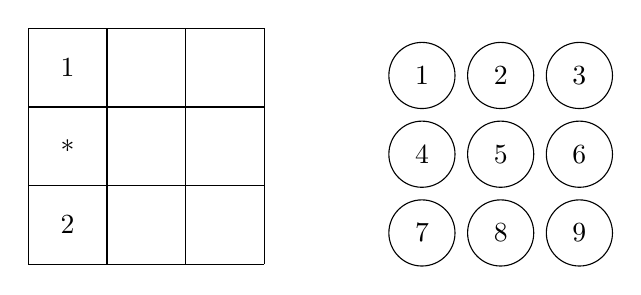
\begin{tikzpicture}[scale=1]
\draw (0,0) grid (3,3);
\node at (0.5,2.5) {$1$};
\node at (0.5,1.5) {$*$};
\node at (0.5,0.5) {$2$};
\foreach \i/\x/\y in {1/5/2.4,2/6/2.4,3/7/2.4,4/5/1.4,5/6/1.4,6/7/1.4,7/5/0.4,8/6/0.4,9/7/0.4}
  \draw (\x,\y) circle (0.42) node {$\i$};
\end{tikzpicture}
\end{center}
\begin{enumerate}[a]
  \item តើគេអាចរៀបកាសទាំង $9$ បានប៉ុន្មានរបៀប?
  \item រកប្រូបាបដែលកាសលេខ $1$ និងលេខ $2$ នៅក្នុងជួរឈរទី $1$ ។
\end{enumerate}
\ans
ក. $9! = 362\,880$ \quad ខ. $\dfrac{3\times 2\times 7!}{9!} = \dfrac{1}{12} \approx 0.083$ ។
\end{pro}

\subsection{គណនាប្រូបាបដោយប្រើបន្សំ}

\begin{example}[លំហាត់គំរូ ១]
គេរើសសិស្ស $8$ នាក់ដោយចៃដន្យក្នុងចំណោមសិស្សប្រុស $9$ នាក់ និងសិស្សស្រី $11$ នាក់ទៅសម្ភាសន៍ ។
\begin{enumerate}[a]
  \item តើគេអាចរៀបសិស្សបានប៉ុន្មានរបៀបខុសៗគ្នា?
  \item រកប្រូបាបនៃព្រឹត្តិការណ៍ ៖\\
  $A$ : “ក្រុមសិស្សទាំង $8$ នាក់មានសុទ្ធតែសិស្សស្រី”\\
  $B$ : “ក្នុងក្រុមមានសិស្សស្រី $5$ នាក់ និងប្រុស $3$ នាក់” ។
\end{enumerate}
\ans
\begin{enumerate}[a]
  \item សកម្មភាពនេះ គឺគេរើសសិស្ស $8$ នាក់ក្នុងចំណោមសិស្ស $20$ នាក់ដោយគ្មានលំដាប់ ហើយសិស្សម្នាក់មិនអាចមានឈ្មោះ $2$ ដងក្នុងក្រុមតែមួយ ។ ចំនួនករណីដែលអាចកើតឡើងជាបន្សំ $8$ ធាតុយកពី $20$ ធាតុ ។ ចំនួនករណីអាចគឺ ${}_{20}C_8 = \dfrac{20!}{12!8!} = 125\,970$ ។
  \item គេរើសសិស្សដោយចៃដន្យ ដូច្នេះធាតុនីមួយៗមានសមប្រូបាប ។
  \begin{itemize}
    \item សិស្ស $8$ នាក់ដែលត្រូវជ្រើសរើសសុទ្ធតែស្រី គឺគេរើស $8$ នាក់ក្នុងចំណោម $11$ នាក់ ។ ចំនួនករណីស្របជាចំនួនបន្សំ ${}_{11}C_8 = 165$ ។ ប្រូបាបនៃព្រឹត្តិការណ៍ $A$ គឺ
    \[
    P(A) = \frac{{}_{11}C_8}{{}_{20}C_8} = \frac{165}{125\,970} \approx 0.0013
    \]
    \item គេរើសសិស្សស្រី $5$ នាក់ និងសិស្សប្រុស $3$ នាក់ចេញពីសិស្សស្រី $11$ នាក់ និងប្រុស $9$ នាក់ ។ ចំនួនរបៀបដែលរើសសិស្សស្រី $5$ នាក់គឺ ${}_{11}C_5$ និងចំនួនរបៀបដែលរើសសិស្សប្រុស $3$ នាក់គឺ ${}_9C_3$ ។ ដូច្នេះ ចំនួនករណីស្របនៃព្រឹត្តិការណ៍ $B$ គឺ ${}_{11}C_5\times{}_9C_3$ ។
    \[
    P(B) = \frac{{}_{11}C_5\times{}_9C_3}{{}_{20}C_8} = \frac{462\times 84}{125\,970} \approx 0.308
    \]
  \end{itemize}
\end{enumerate}
\end{example}

\begin{example}[លំហាត់គំរូ ២]
គេរៀបចំឆ្នោត $150$ សន្លឹកដើម្បីលក់ឱ្យអស់មុនពេលចេញផ្សាយ ដែលក្នុងនោះមានឆ្នោតត្រូវរង្វាន់ $5$ សន្លឹក ។ មនុស្សម្នាក់ទិញឆ្នោត $10$ សន្លឹក ។ រកប្រូបាបដែល ៖
\begin{enumerate}[a]
  \item គ្មានត្រូវរង្វាន់សោះ
  \item ត្រូវរង្វាន់យ៉ាងតិច $1$ សន្លឹក
  \item ត្រូវរង្វាន់ $3$ សន្លឹកគត់ ។
\end{enumerate}
\ans
តាង $A$ : “ជាព្រឹត្តិការណ៍គ្មានត្រូវរង្វាន់សោះ” និង $B$ : “ត្រូវរង្វាន់ $3$ សន្លឹក” ។
\begin{enumerate}[a]
  \item ចំនួនរបៀបដែលអាចទិញឆ្នោតបាន $10$ សន្លឹកគឺ $n(S) = {}_{150}C_{10}$ ជាចំនួនករណីអាច ។ ចំនួនឆ្នោតដែលគ្មានរង្វាន់មាន $150 - 5 = 145$ សន្លឹក ។ ចំនួនរបៀបដែលជ្រើសរើសឆ្នោតគ្មានរង្វាន់ $10$ សន្លឹកគឺ $n(A) = {}_{145}C_{10}$ ជាចំនួនករណីស្រប ។ ដូច្នេះ
  \[
  P(A) = \frac{n(A)}{n(S)} = \frac{{}_{145}C_{10}}{{}_{150}C_{10}} \approx 0.7048
  \]
  \item ព្រឹត្តិការណ៍ត្រូវរង្វាន់យ៉ាងតិច $1$ សន្លឹក ជាព្រឹត្តិការណ៍ផ្ទុយនឹងគ្មានត្រូវរង្វាន់សោះ ។ ប្រូបាបដែលត្រូវរង្វាន់យ៉ាងតិច $1$ សន្លឹកគឺ $P(\bar{A}) = 1 - P(A) \approx 1 - 0.7048 = 0.2952$ ។
  \item ចំនួនរបៀបដែលជ្រើសរើសបានឆ្នោតត្រូវរង្វាន់ $3$ សន្លឹក ក្នុងចំណោមឆ្នោតត្រូវរង្វាន់ $5$ សន្លឹកគឺ ${}_5C_3$ ។ ឯឆ្នោតដែលទិញ $7$ សន្លឹកទៀតជាឆ្នោតគ្មានរង្វាន់ រើសចេញពីឆ្នោត $145$ សន្លឹកដែលគ្មានរង្វាន់ ។ ចំនួនរបៀបដែលជ្រើសរើសបានឆ្នោត $7$ សន្លឹកនេះគឺ ${}_{145}C_7$ ។ គេបាន
  \[
  P(B) = \frac{n(B)}{n(S)} = \frac{{}_5C_3\times{}_{145}C_7}{{}_{150}C_{10}} \approx 0.002
  \]
\end{enumerate}
\end{example}

\begin{pro}
ក្នុងថង់មួយមានអក្សរ $10$ តួ $a, b, c, d, e, f, g, h, i, j$ ។ គេចាប់យកអក្សរ $4$ តួព្រមគ្នាចេញពីថង់ដោយចៃដន្យ ។ រកប្រូបាបដែល ៖
\begin{enumerate}[a]
  \item គ្មានបានស្រៈមួយសោះ
  \item បានស្រៈតែមួយគត់
  \item បានស្រៈតែ $2$ គត់
  \item យ៉ាងតិចណាស់បានស្រៈមួយ ។
\end{enumerate}
\ans
ក. $\dfrac{{}_7C_4}{{}_{10}C_4} = \dfrac{1}{6} \approx 0.167$ \quad ខ. $0.5$ \quad គ. $0.3$ \quad ឃ. $\dfrac{5}{6} \approx 0.833$ ។
\end{pro}

\section*{មេរៀនសង្ខេប ជំពូកទី ៦}
\begin{note}[មេរៀនសង្ខេប]
\begin{enumerate}[1]
  \item \textbf{គោលការណ៍ផលបូក} ៖ $m$ ជាចំនួនធាតុក្នុងព្រឹត្តិការណ៍ $A$ និង $n$ ជាចំនួនធាតុក្នុងព្រឹត្តិការណ៍ $B$ ។
  \begin{itemize}
    \item បើ $A$ និង $B$ ជាព្រឹត្តិការណ៍មិនចុះសម្រុងគ្នា (គ្មានធាតុរួម) នោះព្រឹត្តិការណ៍ $A$ ឬ $B$ មានធាតុ $n(A \cup B) = m + n$ ។
    \item បើ $A$ និង $B$ ជាព្រឹត្តិការណ៍ចុះសម្រុងគ្នា (មាន $p$ ធាតុរួម) នោះព្រឹត្តិការណ៍ $A$ ឬ $B$ មានធាតុ $n(A \cup B) = n(A) + n(B) - n(A \cap B) = m + n - p$ ។
  \end{itemize}
  \item \textbf{គោលការណ៍ផលគុណ}
  \begin{itemize}
    \item បើ $m$ ជាចំនួនធាតុនៃព្រឹត្តិការណ៍ $A$ និង $n$ ជាចំនួនធាតុនៃព្រឹត្តិការណ៍ $B$ កើតឡើងបន្ទាប់ពីព្រឹត្តិការណ៍ $A$ កើតឡើង នោះព្រឹត្តិការណ៍ $A$ និង $B$ កើតឡើងមាន $n(A \cap B) = m\times n$ របៀប ។
    \item ចម្លាស់នៃ $n$ ធាតុ គឺជាការតម្រៀប $n$ វត្ថុខុសៗគ្នាជាជួរមានលំដាប់ ។ ចំនួនចម្លាស់នៃ $n$ ធាតុ មាន ${}_nP_n = n!$ របៀប ៖ $n! = n(n - 1)(n - 2)\cdots 3\times 2\times 1$ ។
    \item ចម្លាស់នៃ $r$ ធាតុយកពី $n$ ធាតុ គឺជាការតម្រៀប $r$ វត្ថុខុសៗគ្នាជាជួរតាមលំដាប់ដែលធាតុនីមួយៗយកចេញពី $n$ ធាតុខុសគ្នា ។ ចំនួនចម្លាស់នៃ $r$ ធាតុយកពី $n$ ធាតុមាន ${}_nP_r = n(n - 1)(n - 2)\cdots(n - r + 1)$ ឬ ${}_nP_r = \dfrac{n!}{(n - r)!}$ $(n \in \mathbb{N}, r \in \mathbb{N}, r \le n)$ ។
    \item ចម្លាស់ច្រំដែលនៃ $r$ ធាតុយកពី $n$ គឺជាការតម្រៀប $r$ ធាតុដែលធាតុនីមួយៗអាចជាធាតុដដែលយកចេញពី $n$ ធាតុខុសគ្នា ។ ចំនួនចម្លាស់ច្រំដែលនៃ $r$ ធាតុយកពី $n$ ធាតុមាន $n^r$ ។
    \item ចំនួនចម្លាស់រង្វង់នៃ $n$ ធាតុមាន $(n - 1)!$ របៀប ។
  \end{itemize}
  \item \textbf{បន្សំ}នៃ $r$ ធាតុយកពី $n$ ធាតុ គឺជាការយក $r$ វត្ថុចេញពី $n$ វត្ថុដោយមិនគិតលំដាប់ ។ ចំនួនបន្សំនៃ $r$ ធាតុយកពី $n$ ធាតុគឺ ${}_nC_r = \dfrac{n!}{(n - r)!r!} = \dfrac{n(n - 1)\cdots(n - r + 1)}{r!}$ ។
  \item \textbf{ទ្រឹស្ដីបទទ្វេធា} ៖ $(a + b)^n = {}_nC_0 a^n + {}_nC_1 a^{n-1}b + {}_nC_2 a^{n-2}b^2 + \dots + {}_nC_n b^n$
  \begin{itemize}
    \item ផលបូកនេះមាន $(n + 1)$ តួ ។
    \item ចំពោះតួបន្តបន្ទាប់គ្នា ស្វ័យគុណរបស់ $a$ ចុះតាមលំដាប់នៅពេលដែលស្វ័យគុណរបស់ $b$ កើនតាមលំដាប់ ។
    \item ក្នុងតួនីមួយៗផលបូកនៃស្វ័យគុណ $a$ និង $b$ ស្មើនឹង $n$ ។
    \item មេគុណរបស់ $a^{n-k}b^k$ គឺ ${}_nC_k$ ។
    \item ករណី $b = 1$ គេបាន $(1 + a)^n = {}_nC_0 + {}_nC_1 a + {}_nC_2 a^2 + \dots + {}_nC_n a^n$ ហើយមេគុណរបស់ $a^k$ គឺ ${}_nC_k$ ។
  \end{itemize}
  \item \textbf{ប្រូបាប}
  \begin{itemize}
    \item ព្រឹត្តិការណ៍ផលគុណនៃ $A$ និង $B$ ជាប្រសព្វនៃព្រឹត្តិការណ៍ $A$ និងព្រឹត្តិការណ៍ $B$ ។
    \item ព្រឹត្តិការណ៍ផលបូកនៃ $A$ និង $B$ ជាប្រជុំនៃព្រឹត្តិការណ៍ $A$ និងព្រឹត្តិការណ៍ $B$ ។
    \item ព្រឹត្តិការណ៍ $B$ និងព្រឹត្តិការណ៍ $D$ ជាព្រឹត្តិការណ៍មិនចុះសម្រុង កាលណាព្រឹត្តិការណ៍ផលគុណនៃ $B$ និង $D$ ជាព្រឹត្តិការណ៍មិនអាចមានគឺ $B \cap D = \varnothing$ ។
    \item ព្រឹត្តិការណ៍ $2$ ជាព្រឹត្តិការណ៍ផ្ទុយគ្នា ឬជាព្រឹត្តិការណ៍បំពេញគ្នា កាលណាព្រឹត្តិការណ៍ផលគុណនៃព្រឹត្តិការណ៍ទាំង $2$ ជាព្រឹត្តិការណ៍មិនអាចមាន និងព្រឹត្តិការណ៍ផលបូកនៃព្រឹត្តិការណ៍ទាំង $2$ ជាព្រឹត្តិការណ៍ប្រាកដដែល $A \cap \bar{A} = \varnothing$, $A \cup \bar{A} = S$ ។ គេបានព្រឹត្តិការណ៍ $2$ បំពេញគ្នាជាព្រឹត្តិការណ៍មិនចុះសម្រុង ។
    \item ប្រូបាបនៃព្រឹត្តិការណ៍មួយ ជាផលធៀបនៃចំនួនករណីស្រប និងចំនួនករណីអាច ៖ $P(A) = \dfrac{\text{ចំនួនករណីស្រប}}{\text{ចំនួនករណីអាច}} = \dfrac{n(A)}{n(S)}$ ។
    \item ប្រូបាបនៃលំហសំណាក $S$ ស្មើនឹង $1$ គឺ $P(S) = 1$ ។ ប្រូបាបនៃព្រឹត្តិការណ៍មិនអាចមានស្មើនឹង $0$ គឺ $P(\varnothing) = 0$ ។
    \item ប្រូបាបនៃព្រឹត្តិការណ៍មួយក្នុងលំហសំណាក ជាចំនួនដែលនៅចន្លោះ $[0, 1]$ ៖ $0 \le P(A) \le 1$ ។
    \item ប្រូបាបនៃព្រឹត្តិការណ៍ផលគុណ $A$ និង $B$ គឺ $P(A \cap B) = P(A)\times P(B)$ បើ $A$ និង $B$ មិនទាក់ទងគ្នា ។ $P(A \cap B) = P(A)\times P(B/A)$ បើ $A$ និង $B$ ទាក់ទងគ្នា ។
    \item ប្រូបាបនៃព្រឹត្តិការណ៍ផលបូក $A$ និង $B$ គឺ $P(A \cup B) = P(A) + P(B) - P(A \cap B)$ ។ $P(A \cup B) = P(A) + P(B)$ កាលណា $A$ និង $B$ ជាព្រឹត្តិការណ៍មិនចុះសម្រុង ។
    \item ប្រូបាបនៃព្រឹត្តិការណ៍បំពេញនៃ $A$ គឺ $P(\bar{A}) = 1 - P(A)$ ។
  \end{itemize}
\end{enumerate}
\end{note}

\section*{លំហាត់ជំពូកទី ៦}
\begin{enumerate}[1]
  \item គណនា ៖
  \begin{tasks}(5)
    \task $8!$
    \task $10!$
    \task $0!$
    \task $1!$
    \task ${}_7P_5$
    \task ${}_{12}P_4$
    \task ${}_5P_3$
    \task ${}_6P_0$
    \task ${}_5P_5$
    \task ${}_6P_2$
  \end{tasks}
  \item គណនា ៖
  \begin{tasks}(5)
    \task ${}_5C_2$
    \task ${}_8C_3$
    \task ${}_6C_2$
    \task ${}_6C_4$
    \task ${}_3C_3$
    \task ${}_9C_7$
    \task ${}_4C_3$
    \task ${}_{12}C_2$
    \task ${}_7C_4$
    \task ${}_3C_0$
  \end{tasks}
  \item ដោះស្រាយសមីការ ៖
  \begin{tasks}(3)
    \task ${}_nP_2 = 56$
    \task ${}_nP_2 = 60$
    \task ${}_nP_2 = 30$
    \task ${}_nP_3 = 990$
    \task $2({}_nP_2) = 60$
  \end{tasks}
  \item ដោះស្រាយសមីការ ៖
  \begin{tasks}(4)
    \task ${}_8P_r = 3!$
    \task ${}_7P_r = 7!$
    \task ${}_nP_2 = 4({}_{n-1}P_2)$
    \task $n({}_nP_3) = {}_nP_6$
  \end{tasks}
  \item សម្រួលកន្សោម ៖
  \begin{tasks}(2)
    \task $\dfrac{3!(n + 2)!}{4!(n - 1)!}$
    \task $\dfrac{7!(r - 1)!}{6!(r + 1)!} + \dfrac{5!r!}{3!(r + 1)!}$
    \task $\dfrac{{}_nC_5}{{}_{n-1}C_3}$
    \task $({}_{n-1}C_3)\left(\dfrac{1}{{}_{n-2}C_3}\right)$
  \end{tasks}
  \item ដោះស្រាយសមីការ ៖
  \begin{tasks}(3)
    \task $2({}_nC_2) = {}_{n+1}C_3$
    \task ${}_nC_1 = 10$
    \task ${}_nC_2 = 21$
    \task ${}_nC_2 = 28$
    \task ${}_{n+1}C_{n-1} = 15$
    \task ${}_nC_{n-2} = 6$
    \task $720({}_nC_5) = {}_{n+1}P_5$
    \task ${}_nC_3 = 4({}_nP_2)$
  \end{tasks}
  \item នៅអាហារដ្ឋានមានរៀបឈុតអាហារសម្រាប់បម្រើសេចក្ដីត្រូវការរបស់ភ្ញៀវមួយពេល ។ មួយឈុតអាហារមាន បាយ សាច់ បន្លែ និងភេសជ្ជៈ ។ សម្រាប់បាយមានបីប្រភេទគឺ បាយ មី និងដំឡូងបារាំង សម្រាប់សាច់មាន សាច់គោ ជ្រូក ត្រី មាន់ សម្រាប់បន្លែមាន សណ្ដែក ការ៉ុត ប៉េងប៉ោះ និងភេសជ្ជៈមាន កូកាកូឡា សាស៊ី ទឹកផ្លែឈើ ស្រាបៀរ ។ តើគេអាចបង្កើតឈុតម្ហូបបានប៉ុន្មានរបៀប?
  \item រកចំនួនពាក្យ (ពាក្យមានន័យឬពាក្យគ្មានន័យ) ដែលកើតឡើងពីតួអក្សរនៃពាក្យ ៖ \quad ក. $SIMPLE$ \quad ខ. $SECONDARY$ ។
  \item ក្នុងចំណោមសិស្សប្រុស $5$ នាក់ និងស្រី $8$ នាក់ ដែលមានស្នាដៃល្អក្នុងការតែងកំណាព្យ គ្រូជ្រើសរើសសិស្សប្រុស $3$ នាក់ និងស្រី $4$ នាក់ឡើងបង្ហាញស្នាដៃតាមលំដាប់មុនក្រោយ ។ តើគ្រូអាចជ្រើសរើសសិស្សទាំងនេះបានប៉ុន្មានរបៀប?
  \item បងប្អូនប្រុស $3$ នាក់ និងស្រី $2$ នាក់ឈរជាជួរថតរូប ។ តើគេឈរបានប៉ុន្មានរបៀប បើមានក្មេងប្រុស $2$ នាក់ឈរចុងសងខាង ។
  \item រកចំនួននៃការតម្រៀបតួអក្សររបស់ពាក្យ $INCLUDE$ បើ ៖
  \begin{enumerate}[a]
    \item គ្រប់ព្យញ្ជនៈនៅជាប់គ្នា
    \item គ្មានព្យញ្ជនៈ $2$ ណានៅជាប់គ្នា
    \item ការតម្រៀបនីមួយៗ ចាប់ផ្ដើមដោយព្យញ្ជនៈ និងបញ្ចប់ដោយស្រៈ ។
  \end{enumerate}
  \item រកចំនួននៃចំនួនដែលនៅចន្លោះ $2000$ និង $5000$ ហើយមានលេខខុសៗគ្នា ដោយប្រើលេខ $1, 2, 4, 5, 7$ និង $8$ ។
  \item នៅលើថតទូមួយមានតម្រៀបសៀវភៅ គណិតវិទ្យា $4$ រូបវិទ្យា $3$ និងគីមីវិទ្យា $2$ ។ តើគេអាចរៀបបានប៉ុន្មានរបៀបបើ ៖
  \begin{enumerate}[a]
    \item សៀវភៅរូបវិទ្យា $3$ នៅជាប់គ្នា
    \item សៀវភៅគីមីវិទ្យាមិននៅជាប់គ្នា
    \item សៀវភៅរូបវិទ្យាមិននៅជាប់គ្នា ។
  \end{enumerate}
  \item ក្មេងប្រុស $4$ នាក់ និងក្មេងស្រី $5$ នាក់ឈរតម្រៀបគ្នាជាជួរ ។
  \begin{enumerate}[a]
    \item រកចំនួនរបៀបដែលអាចឈរបាន
    \item រកចំនួនរបៀបឈរ បើ ៖ $2$ នាក់ដំបូងជាក្មេងស្រី ។ ម្នាក់ដំបូងជាក្មេងប្រុស និងម្នាក់ខាងចុងជាក្មេងស្រី ។ ក្មេងប្រុសនៅឈរជិតគ្នា ។ គ្មានក្មេងស្រីណាឈរជិតគ្នា ។
  \end{enumerate}
  \item ហាងមួយមានអាវយឺត $7$ ពណ៌សុទ្ធតែជាពណ៌ដែលសុខចូលចិត្តទាំងអស់ ប៉ុន្តែសុខមានប្រាក់ទិញបានត្រឹមតែអាវយឺត $3$ ប៉ុណ្ណោះ ។ តើសុខមានជម្រើសប៉ុន្មានរបៀប ដើម្បីយកអាវយឺត $3$ នេះ?
  \item ក្រុមកីឡាករមានមនុស្ស $10$ នាក់ ដែលមានស្ត្រី $4$ នាក់ និងបុរស $6$ នាក់ ។ គេរើសកីឡាករ $4$ នាក់ ដើម្បីធ្វើការប្រកួតគ្នា ។ រកចំនួនរបៀបដែលជ្រើសរើស បើ ៖
  \begin{enumerate}[a]
    \item កីឡាករត្រូវប្រកួតមានភេទដូចគ្នា
    \item កីឡាករត្រូវប្រកួតមានចំនួនស្រីស្មើនឹងបុរស ។
    \item ក្រុមប្រកួតមានបុរសឈ្មោះ $A$ ឬក្រុមមានបុរសឈ្មោះ $B$ ប៉ុន្តែមិនមែនជាក្រុមមានបុរសឈ្មោះ $A$ និង $B$ ។
  \end{enumerate}
  \item មានសិស្ស $10$ នាក់ស្ម័គ្រចិត្តចូលរួមក្នុងការងារសង្គមរបស់សហគមន៍ ។ ប្រធានសហគមន៍ចែកសិស្ស $5$ នាក់ ចុះតាមភូមិដើម្បីផ្ដល់ប្រឹក្សាដល់ប្រជាជន $3$ នាក់ជួយកិច្ចការរដ្ឋបាល និង $2$ នាក់ចុះស្រង់ពត៌មាន ។ តើប្រធានអាចចែកសិស្សតាមក្រុមបានប៉ុន្មានរបៀប?
  \item គេជ្រើសរើសសិស្ស $5$ នាក់ក្នុងចំណោមសិស្សស្រី $7$ នាក់ និងសិស្សប្រុស $10$ នាក់ឱ្យចូលរួមប្រជុំការងារ ។ តើគេអាចរើសសិស្ស $5$ នាក់នេះបានប៉ុន្មានរបៀបបើ ៖
  \begin{enumerate}[a]
    \item គ្មានលក្ខខណ្ឌ?
    \item មានសិស្សស្រី $3$ នាក់ និងប្រុស $2$ នាក់?
    \item មានសិស្សស្រីយ៉ាងតិចម្នាក់?
  \end{enumerate}
  \item ក្នុងកម្រងសំណួរពហុជ្រើសរើសមាន $5$ សំណួរដែលសំណួរនីមួយៗមានចម្លើយ $3$ ។ គេអាចជ្រើសរើសយកចម្លើយបានតែមួយគត់ក្នុងមួយសំណួរ ។ តើគេអាចបានកម្រងចម្លើយប៉ុន្មានរបៀបខុសគ្នា?
  \item រកមេគុណរបស់ $x^4$ និង $x^5$ ក្នុងការពន្លាតទ្វេធានៃ $\left(1 - \dfrac{x}{2}\right)^{12}$ ។
  \item រកមេគុណរបស់ $x^2$ ក្នុងការពន្លាតកន្សោម $(1 - 2x)^5(1 + 3x)^9$ ។
  \item បង្ហាញថា ${}_nC_0 - {}_nC_1 + {}_nC_2 - {}_nC_3 + \dots + (-1)^n{}_nC_n = 0$ ។
  \item សរសេរ $4$ តួដំបូងតាមស្វ័យគុណកើននៃ $y$ ក្នុងការពន្លាតទ្វេធានៃកន្សោម ៖ \quad ក. $(1 - 3y)^8$ \quad ខ. $\left(1 + \dfrac{3y}{3}\right)^8$ ។
  \item គេពន្លាតទ្វេធានៃកន្សោមនីមួយៗខាងក្រោម ៖
  \begin{enumerate}[a]
    \item រកតួដែលមាន $x^{12}$ ក្នុងលទ្ធផលពន្លាតកន្សោម $(1 + 2x^2)^8$ ។
    \item រកតួដែលមាន $x^3$ ក្នុងលទ្ធផលពន្លាតកន្សោម $\left(x - \dfrac{2}{x^2}\right)^{12}$ ។
  \end{enumerate}
  \item រកមេគុណនៃ $x^6$ និង $x^8$ ក្នុងលទ្ធផលពន្លាតទ្វេធា $\left(1 + \dfrac{1}{2}x^2\right)^{10}$ ។ ទាញរកមេគុណនៃ $x^8$ ក្នុងលទ្ធផលពន្លាតទ្វេធានៃ $(2x^2 + 3)\left(1 + \dfrac{1}{2}x^2\right)^{10}$ ។
  \item ក្នុងការពន្លាតទ្វេធាខាងក្រោមនេះ ចូរសរសេរតួទី $7$ រាប់តាមលំដាប់ស្វ័យគុណកើននៃ $x$ ៖ \quad ក. $\left(2 + \dfrac{x^2}{2}\right)^{11}$ \quad ខ. $\left(2x - \dfrac{1}{x^2}\right)^{12}$ ។
  \item ក្នុងកម្រងបទចម្រៀង $10$ បទ ដែល $5$ បទជាចម្រៀងរបស់លោកស៊ីន ស៊ីសាមុត $3$ បទជារបស់លោកស្រីរស់ សេរីសុទ្ធា និង $2$ បទជាចម្រៀងរបស់អ្នកនាងហួយ មាស ។ គេចង់ជ្រើសរើសចម្រៀង $4$ បទ ដើម្បីច្រៀងកំដរអារម្មណ៍ក្នុងពិធីជប់លៀងមួយ ។ តើគេអាចជ្រើសរើសចម្រៀង $4$ បទនេះបានប៉ុន្មានរបៀបបើ ៖
  \begin{enumerate}[a]
    \item មិនប្រកាន់ជាបទរបស់អ្នកណា?
    \item $2$ បទជារបស់លោកស៊ីន ស៊ីសាមុត $1$ បទជារបស់លោកស្រីរស់ សេរីសុទ្ធា និង $1$ បទជារបស់អ្នកនាងហួយ មាស?
    \item យ៉ាងតិចមានមួយបទម្នាក់?
    \item ជាបទចម្រៀងរបស់ម្ចាស់ដើមតែ $2$ នាក់គត់?
  \end{enumerate}
  \item រកប្រូបាបនៃការបោះគ្រាប់ឡុកឡាក់ពីរគ្រាប់តាមករណីដែលគេទទួលបានដូចខាងក្រោម ៖
  \begin{tasks}(3)
    \task ផលបូកស្មើ $6$ ឬ $7$
    \task ផលបូកធំជាង $8$
    \task ផលបូកតូចជាង $3$ ឬធំជាង $8$
    \task ផលបូកស្មើ $16$
    \task ផលបូកតិចជាង $11$ ។
  \end{tasks}
  \item គ្រាប់ឡុកឡាក់ $1$ គ្រាប់មានមុខ $6$ ដែលមុខនីមួយៗមានចុះលេខ $1, 2, 3, 5, 8$ និង $13$ ។
  \begin{enumerate}[a]
    \item បើគេបោះគ្រាប់ឡុកឡាក់មួយដង តើប្រូបាបដែលគេទទួលបានលេខសេសស្មើប៉ុន្មាន?
    \item បើគេបោះគ្រាប់ឡុកឡាក់ពីរដង និងគេបូកលេខវា តើប្រូបាបដែលគេទទួលបានផលបូកជាចំនួនគូស្មើប៉ុន្មាន?
  \end{enumerate}
  \item គេបោះកាក់មួយគ្រាប់ និងហូតបៀមួយសន្លឹកចេញពីបៀមួយហ៊ូ ។ រកប្រូបាបដែលគេអាចទទួលបាន ៖
  \begin{tasks}(2)
    \task ក្បាលនិងសន្លឹកលេខ $6$
    \task កន្ទុយនិងសន្លឹកក្រហម
    \task ក្បាលនិងសន្លឹកជួង
    \task កន្ទុយនិងសន្លឹករូប ។
  \end{tasks}
  \item រកប្រូបាបដែលគេហូតបានសន្លឹករូបពីរសន្លឹក ពេលដែលគេហូតសន្លឹកបៀពីរសន្លឹកចេញពីបៀមួយហ៊ូដោយមិនដាក់ទៅវិញ ។
  \item គេបានលក់សំបុត្រចំនួន $50$ សន្លឹក ដែលមានសន្លឹករង្វាន់ចំនួនពីរសន្លឹក ។ ចូររកប្រូបាបដែលបុរសម្នាក់នឹងឈ្នះពីររង្វាន់ បើបុរសនោះបានទិញសំបុត្រពីរសន្លឹក ។
  \item គេបង្កើតគណៈកម្មការគ្រូនិងមាតាបិតាសិស្សមួយ ដែលមានគ្នា $4$ នាក់ ដោយរើសចេញពីគ្រូ $5$ នាក់ និងមាតាបិតាសិស្សចំនួន $20$ នាក់ ។ ចូររកប្រូបាបដែលគេអាចរើសគណៈកម្មការមានសមាសភាពតាមករណីដូចខាងក្រោម ៖
  \begin{tasks}(2)
    \task គ្រូទាំងអស់
    \task គ្រូ $2$ នាក់និងមាតាបិតា $2$ នាក់
    \task មាតាបិតាទាំងអស់
    \task គ្រូម្នាក់និងមាតាបិតា $3$ នាក់ ។
  \end{tasks}
  \item ក្រុមហ៊ុនមួយមានអ្នកគ្រប់គ្រងចំនួន $7$ នាក់ក្នុងនោះមានស្ត្រីចំនួន $4$ នាក់ ។ គេរើសអ្នកគ្រប់គ្រងចំនួន $3$ នាក់មកចូលរួមក្នុងវគ្គបណ្ដុះបណ្ដាល ។ ចូររកប្រូបាបដែលគេអាចរើសបានតាមករណីដូចខាងក្រោម ៖
  \begin{tasks}(2)
    \task ស្ត្រីទាំងអស់
    \task បុរសទាំងអស់
    \task បុរស $2$ នាក់និងស្ត្រី $1$ នាក់
    \task យ៉ាងហោចណាស់មានស្ត្រី $2$ នាក់
    \task យ៉ាងច្រើនមានបុរស $2$ នាក់ ។
  \end{tasks}
\end{enumerate}

\section*{លំហាត់អនុវត្តន៍}
\begin{enumerate}[1]
  \item គេបោះកាក់មួយ និងគ្រាប់ឡុកឡាក់មួយគ្រាប់ព្រមគ្នា ។ ចូរកំណត់ ៖ \quad ក. សកម្មភាពដែលជាពិសោធន៍ចៃដន្យ និងជាវិញ្ញាសា ។ \quad ខ. លំហសំណាក $S$ និងព្រឹត្តិការណ៍ $A$ : “បោះកាក់បានខាងរូប $H$” និង $B$ : “បោះគ្រាប់ឡុកឡាក់បានលេខ $4$” ។ \quad គ. រកប្រូបាបព្រឹត្តិការណ៍ផ្ទុយនឹង $A$ ព្រឹត្តិការណ៍ផ្ទុយនឹង $B$ និងព្រឹត្តិការណ៍ផលគុណ $A$ និង $B$ ។
  \ans
  ក. ពិសោធន៍ចៃដន្យ ៖ ការបោះកាក់ និងគ្រាប់ឡុកឡាក់ ។ វិញ្ញាសា ៖ ការបោះកាក់មួយ និងគ្រាប់ឡុកឡាក់មួយព្រមគ្នាម្ដង ។ \quad ខ. $S = \{H1, H2, H3, H4, H5, H6, T1, T2, T3, T4, T5, T6\}$, $n(S) = 12$ ។ $A = \{H1, \dots, H6\}$, $B = \{H4, T4\}$ ។ \quad គ. $P(\bar{A}) = \dfrac{1}{2}$, $P(\bar{B}) = \dfrac{5}{6}$, $P(A \cap B) = \dfrac{1}{12}$ ។
  \item គេហូតបៀមួយសន្លឹកដោយចៃដន្យចេញពីហ៊ូបៀរ $52$ សន្លឹក ។ រកប្រូបាបដែលហូតបាន ៖ \quad ក. សន្លឹកអាត់ \quad ខ. សន្លឹកក្រហម \quad គ. សន្លឹកអាត់ឬក្រហម \quad ឃ. មិនមែនអាត់និងមិនមែនក្រហម ។
  \ans
  ក. $\dfrac{4}{52} = \dfrac{1}{13}$ \quad ខ. $\dfrac{26}{52} = \dfrac{1}{2}$ \quad គ. $\dfrac{4 + 26 - 2}{52} = \dfrac{7}{13}$ \quad ឃ. $1 - \dfrac{7}{13} = \dfrac{6}{13}$ ។
  \item ថង់មួយមានឃ្លី $10$ ចុះលេខពី $0$ ដល់ $9$ ។ គេចាប់យកឃ្លីមួយដោយចៃដន្យ ។ ចូរកំណត់ ៖ \quad ក. លំហសំណាក $S$ និងព្រឹត្តិការណ៍ $A$ : “ចាប់បានឃ្លីមានលេខជាពហុគុណនៃ $3$” និង $B$ : “ចាប់បានឃ្លីមានលេខធំជាង $5$” ។ \quad ខ. រកប្រូបាបនៃព្រឹត្តិការណ៍ $A, B, A \cap B$ និង $A \cup B$ ។
  \ans
  ក. $S = \{0, 1, 2, \dots, 9\}$, $A = \{0, 3, 6, 9\}$ ($0$ ក៏ជាពហុគុណនៃ $3$), $B = \{6, 7, 8, 9\}$ ។ \quad ខ. $P(A) = \dfrac{2}{5}$, $P(B) = \dfrac{2}{5}$, $A \cap B = \{6, 9\}$ ៖ $P(A \cap B) = \dfrac{1}{5}$, $P(A \cup B) = \dfrac{2}{5} + \dfrac{2}{5} - \dfrac{1}{5} = \dfrac{3}{5}$ ។
  \item ថង់មួយមានឃ្លីខៀវ $7$ និងឃ្លីស $3$ ។ គេចាប់យកឃ្លីម្ដង $3$ ដោយចៃដន្យតែម្ដងគត់ ។ រកប្រូបាបដែលចាប់បាន ៖ \quad ក. ឃ្លីខៀវ $2$ និងឃ្លីស $1$ \quad ខ. ឃ្លីខៀវទាំង $3$ \quad គ. ឃ្លីសទាំង $3$ ។
  \ans
  $n(S) = {}_{10}C_3 = 120$ ។ ក. $\dfrac{{}_7C_2\times 3}{120} = \dfrac{63}{120} = \dfrac{21}{40}$ \quad ខ. $\dfrac{{}_7C_3}{120} = \dfrac{35}{120} = \dfrac{7}{24}$ \quad គ. $\dfrac{1}{120}$ ។
  \item គេបោះគ្រាប់ឡុកឡាក់ $2$ ព្រមគ្នា មួយពណ៌ខៀវ មួយទៀតពណ៌ក្រហម ។ រកប្រូបាបដែល ៖ \quad ក. លេខចេញលើគ្រាប់ខៀវ ស្មើនឹង $2$ ដងនៃលេខចេញលើគ្រាប់ក្រហម \quad ខ. ផលបូកលេខគ្រាប់ឡុកឡាក់ទាំង $2$ ស្មើនឹង $5$ ។
  \ans
  $n(S) = 36$ ។ ក. (ខៀវ, ក្រហម) $= (2, 1), (4, 2), (6, 3)$ ៖ $P = \dfrac{3}{36} = \dfrac{1}{12}$ \quad ខ. $(1,4), (2,3), (3,2), (4,1)$ ៖ $P = \dfrac{4}{36} = \dfrac{1}{9}$ ។
  \item ក្នុងប្រអប់ $1$ មានក្រដាសបត់ជាសន្លឹកឆ្នោតចាប់យករង្វាន់ ។ សន្លឹកឆ្នោតមាន $20$ សន្លឹកដែលឆ្នោតត្រូវរង្វាន់មាន $12$ សន្លឹកសម្រាប់សិស្ស $20$ នាក់ចាប់យកមួយសន្លឹកម្នាក់បន្តបន្ទាប់គ្នា ដើម្បីផ្ទៀងមើលរង្វាន់រៀងៗខ្លួន ។ សុខជាអ្នកចាប់បានមុនគេ បន្ទាប់មកសោចាប់ទី $2$ និងសនចាប់ទី $3$ និងសិស្សឯទៀតចាប់ម្នាក់មួយបន្តបន្ទាប់គ្នារហូតអស់ឆ្នោត ។ រកប្រូបាបដែល ៖ \quad ក. សុខចាប់បានឆ្នោតត្រូវរង្វាន់ \quad ខ. សោចាប់បានឆ្នោតត្រូវរង្វាន់ \quad គ. សនចាប់បានឆ្នោតត្រូវរង្វាន់ \quad ឃ. តើអ្នកចាប់មុននិងអ្នកចាប់ក្រោយអ្នកណាមានសំណាងជាងអ្នកណា?
  \ans
  ក. $\dfrac{12}{20} = \dfrac{3}{5}$ \quad ខ. $\dfrac{12}{20}\times\dfrac{11}{19} + \dfrac{8}{20}\times\dfrac{12}{19} = \dfrac{3}{5}$ \quad គ. $\dfrac{3}{5}$ \quad ឃ. សំណាងស្មើគ្នា ($\dfrac{3}{5}$ ដូចគ្នា) មិនអាស្រ័យនឹងលំដាប់ចាប់ទេ ។
\end{enumerate}
